\documentclass[12pt,a4paper]{report}

\usepackage[a4paper,left=3cm,right=2cm,top=2.5cm,bottom=2.5cm]{geometry}
\usepackage{fontspec}
\usepackage{polyglossia}
\setmainlanguage{vietnamese}
\setmainfont{Noto Serif}
\setsansfont{Noto Sans}
\usepackage{amsmath,amssymb}
\usepackage{booktabs}
\usepackage{longtable}
\usepackage{array}
\usepackage{tabularx}
\usepackage{enumitem}
\usepackage{graphicx}
\usepackage{float}
\usepackage{caption}
\usepackage{subcaption}
\usepackage{xcolor}
\usepackage{hyperref}
\usepackage{listings}
\usepackage{fancyhdr}
\usepackage{titlesec}
\usepackage{tikz}
\graphicspath{{images/}}

\hypersetup{
	colorlinks=true,
	linkcolor=black,
	urlcolor=blue,
	citecolor=black
}

\pagestyle{fancy}
\fancyhf{}
\fancyhead[L]{OISM -- Báo cáo đồ án Capstone Project}
\fancyhead[R]{\thepage}
\renewcommand{\headrulewidth}{0.4pt}

\setlength{\parindent}{1cm}
\setlength{\parskip}{0.4em}
\renewcommand{\arraystretch}{1.3}

\lstset{
	basicstyle=\ttfamily\small,
	breaklines=true,
	frame=single,
	columns=fullflexible,
	keepspaces=true
}

\begin{document}
	
	% ============================================================
	% BÌA
	% ============================================================
	\begin{titlepage}
		\thispagestyle{empty}
		\centering
		
		{\large\bfseries MINISTRY OF CONSTRUCTION\par}
		\vspace{0.35cm}
		{\large\bfseries UNIVERSITY OF TRANSPORT AND COMMUNICATIONS HO CHI MINH CITY\par}
		\vspace{0.35cm}
		{\large\bfseries FACULTY OF INFORMATION TECHNOLOGY\par}
		
		\vspace{0.8cm}
		
		\begin{center}
			
\includegraphics[width=0.45\textwidth]{logo_full.png}
			\vspace{0.4cm}
		\end{center}
		
		\vspace{0.3cm}
		
		{\fontsize{22}{26}\selectfont
			\bfseries Capstone Project Document\par}
		\vspace{0.3cm}
		{\large \textbf{Omnichannel Inventory and Sales Management System (OISM)}\par}
		
		\vspace{0.65cm}
		\noindent\rule{0.86\textwidth}{0.5pt}
		\vspace{0.45cm}
		
		\begin{tabular}{|p{0.93\textwidth}|}
			\hline
			\begin{tabular}{@{}p{0.29\textwidth}@{}p{0.61\textwidth}@{}}
				\bfseries Group Members &
				Phan Quỳnh Thanh Hải - 079205041771\\
				& Phan Trung Kiên - 052206000365\\
				& Lê Phương Ngân - 083306004468\\
				& Hoàng Nguyễn Quỳnh Như - 064306002448\\
				& Nguyễn Hữu Nghĩa - 056207010361\\
			\end{tabular}\\
			\hline
			\begin{tabular}{@{}p{0.29\textwidth}@{}p{0.61\textwidth}@{}}
				\bfseries Supervisor & Nguyễn Văn Chiến\\
			\end{tabular}\\
			\hline
			\begin{tabular}{@{}p{0.29\textwidth}@{}p{0.61\textwidth}@{}}
				\bfseries Capstone Project Code & OISM2\\
			\end{tabular}\\
			\hline
		\end{tabular}
		
		\vfill
		
		{\large - Ho Chi Minh City, September 2026 -\par}
	\end{titlepage}
	
	% ============================================================
	% LỜI CẢM ƠN
	% ============================================================
	\chapter*{LỜI CẢM ƠN}
	\addcontentsline{toc}{chapter}{LỜI CẢM ƠN}
	Đồ án tốt nghiệp với đề tài \textit{Omnichannel Inventory and Sales Management System (OISM)} là cột mốc quan trọng đánh dấu chặng đường học tập, rèn luyện và nghiên cứu chuyên sâu của nhóm sinh viên chúng em tại Khoa Công nghệ Thông tin - Trường Đại học Giao thông Vận tải Phân hiệu tại TP.HCM (UTH). Để hoàn thành công trình này, nhóm xin bày tỏ lòng biết ơn sâu sắc đến giảng viên hướng dẫn - Thầy Nguyễn Văn Chiến, người đã tận tình định hướng chuyên môn, truyền đạt những kinh nghiệm thực tiễn quý báu và trực tiếp đồng hành cùng nhóm qua từng giai đoạn phát triển của dự án.
	
	Trong quá trình nghiên cứu và hiện thực hóa đề tài, nhóm đã tiếp thu được lượng kiến thức vô giá về quy trình phát triển phần mềm chuẩn doanh nghiệp, kiến trúc hướng sạch (Clean Architecture), mô hình cơ sở dữ liệu phân tán SaaS đa thuê bao, cũng như các kỹ thuật xử lý đồng thời mức độ cao nhằm giải quyết bài toán chống bán quá tải trong thương mại điện tử. 
	
	Chúng em xin gửi lời tri ân sâu sắc đến gia đình, bạn bè và nhà trường đã tạo mọi điều kiện thuận lợi nhất để nhóm hoàn thành tốt quãng thời gian học tập và thực hiện Capstone Project.
	
	\vspace{1.5cm}
	\begin{flushright}
		\textit{Nhóm sinh viên thực hiện}
	\end{flushright}
	
	% ============================================================
	% DANH MỤC TỪ VIẾT TẮT
	% ============================================================
	\chapter*{DANH MỤC TỪ VIẾT TẮT}
	\addcontentsline{toc}{chapter}{DANH MỤC TỪ VIẾT TẮT}
	\begin{longtable}{p{0.25\textwidth}p{0.65\textwidth}}
		\toprule
		\textbf{Từ viết tắt} & \textbf{Ý nghĩa}\\
		\midrule
		OISM & Omnichannel Inventory and Sales Management System\\
		POS & Point of Sale (Điểm bán hàng trực tiếp tại quầy)\\
		SKU & Stock Keeping Unit (Mã phân loại đơn vị lưu kho sản phẩm)\\
		COGS & Cost of Goods Sold (Giá vốn hàng bán thực tế)\\
		WAC & Weighted Average Cost (Phương pháp tính giá vốn bình quân gia quyền)\\
		RBAC & Role-Based Access Control (Cơ chế phân quyền dựa trên vai trò người dùng)\\
		JWT & JSON Web Token (Mã thông báo định danh bảo mật web JSON)\\
		API & Application Programming Interface (Giao diện lập trình ứng dụng hệ thống)\\
		SaaS & Software as a Service (Mô hình cung cấp phần mềm ứng dụng dạng dịch vụ đám mây)\\
		PWA & Progressive Web Application (Ứng dụng web tiến bộ di động/máy tính)\\
		\bottomrule
	\end{longtable}
	
	% ============================================================
	% DANH MỤC HÌNH, BẢNG & MỤC LỤC
	% ============================================================
	\tableofcontents
	\listoffigures
	\listoftables
	
	% ============================================================
	% CHƯƠNG 1. GIỚI THIỆU ĐỀ TÀI
	% ============================================================
	\chapter{GIỚI THIỆU ĐỀ TÀI}
	\section{Tổng quan dự án}
	Hệ thống Quản lý Bán hàng và Tồn kho Đa kênh (OISM) được nghiên cứu và phát triển nhằm thiết lập một hạ tầng phần mềm tập trung, cho phép các doanh nghiệp bán lẻ quy mô vừa và lớn quản lý đồng bộ toàn bộ chuỗi cung ứng sản phẩm, đơn hàng và dòng tiền trên một nền tảng duy nhất. Dự án kết hợp chặt chẽ giữa các nguyên lý kiến trúc phần mềm hướng sạch (Clean Architecture) và mô hình phân phối phần mềm dịch vụ đa thuê bao (SaaS Multi-tenant), đảm bảo tính cô lập dữ liệu tuyệt đối giữa các cửa hàng độc lập nhưng vẫn tối ưu hóa khả năng vận hành hệ thống.
	
	\section{Bối cảnh bài toán}
	Sự bùng nổ mạnh mẽ của thương mại điện tử và mô hình kinh doanh O2O (Online-to-Offline) đòi hỏi các doanh nghiệp bán lẻ phải hiện diện đồng thời trên nhiều kênh phân phối khác nhau: từ hệ thống cửa hàng vật lý truyền thống (POS) đến các gian hàng trực tuyến trên các sàn thương mại điện tử lớn như Shopee, Lazada hay TikTok Shop. Sự phân mảnh này dẫn đến thực tế là các nhà quản lý phải đối mặt với áp lực cực lớn trong việc giữ cho dữ liệu hàng hóa giữa các kênh luôn ở trạng thái thời gian thực.
	
	\section{Các vấn đề của hệ thống hiện tại}
	Thông qua khảo sát thực tế tại các mô hình bán lẻ đang vận hành thủ công hoặc sử dụng các phần mềm rời rạc, nhóm ghi nhận ba điểm nghẽn chí mạng sau:
	\begin{itemize}
		\item \textbf{Hiện tượng Overselling (Bán quá tải):} Độ trễ trong quá trình đồng bộ tồn kho giữa kênh online và offline khiến hệ thống vẫn tiếp tục nhận đơn hàng đặt mua từ khách hàng trong khi số lượng sản phẩm thực tế trong kho vật lý đã hoàn toàn cạn kiệt.
		\item \textbf{Sai lệch dữ liệu tồn kho:} Các thao tác điều chỉnh, nhập xuất kho thực hiện bằng phương pháp thủ công dễ sinh ra thất thoát, sai số số liệu giữa sổ sách và thực tế nhưng không thể truy vết nguyên nhân.
		\item \textbf{Khó khăn trong việc tính toán COGS:} Giá nhập hàng từ nhà cung cấp biến động liên tục theo thời gian và theo từng lô hàng, làm sai lệch nghiêm trọng biên lợi nhuận gộp của doanh nghiệp nếu không có cơ chế tự động hóa ghi nhận.
	\end{itemize}
	
	\section{Các hệ thống tương tự}
	Đồ án đã tiến hành phân tích sâu các giải pháp quản lý bán hàng hiện hành trên thị trường. Các hệ thống này tuy mạnh về giao diện trực quan nhưng thường gặp hạn chế về khả năng xử lý đồng thời khi gặp các sự kiện Flash Sale lớn. OISM ra đời khắc phục triệt để nhược điểm đó bằng mô hình sổ cái tồn kho bất biến (\textit{Inventory Ledger}).
	
	\section{Cơ hội kinh doanh}
	Thị trường bán lẻ Việt Nam đang bước vào giai đoạn chuyển đổi số toàn diện. Việc cung cấp một hệ thống SaaS đa thuê bao tối ưu chi phí đầu tư hạ tầng, tự động hóa toàn bộ quy trình kho và bán hàng mở ra cơ hội thương mại hóa lớn cho sản phẩm.
	
	\section{Tầm nhìn sản phẩm}
	Trở thành hệ sinh thái công nghệ tin cậy, giúp doanh nghiệp loại bỏ hoàn toàn tình trạng overselling, tự động hóa hoàn toàn phép tính giá vốn hàng bán và minh bạch hóa toàn bộ chuỗi giá trị bán lẻ.
	
	\section{Phạm vi đề tài}
	Phạm vi nghiên cứu tập trung vào các phân hệ trọng tâm: Quản lý Tenant \& Xác thực bảo mật (FR-AUTH), Quản lý danh mục sản phẩm và biến thể SKU (FR-PROD), Sổ cái tồn kho bất biến không cho phép sửa xóa (FR-INV), Tự động tính toán giá vốn bình quân gia quyền WAC (FR-COST), Hub điều phối đơn hàng tập trung (FR-ORD), Cơ chế giữ chỗ chống bán vượt (FR-RSE), Giao diện bán hàng PWA POS (FR-POS), Hệ thống báo cáo phân tích (FR-REP) và Trình giả lập Webhook thương mại điện tử (FR-SIM).
	
	\section{Giới hạn đề tài}
	Hệ thống hiện tại tập trung giải quyết bài toán thương mại bán lẻ đa kênh thuần túy, chưa tích hợp sâu với các cơ quan quản lý thuế nhà nước hoặc các cổng thanh toán quốc tế phức tạp; các tính năng dự báo thông minh dựa trên AI vận hành trên cơ sở dữ liệu mô phỏng trong phạm vi đồ án.
	
	% ============================================================
	% CHƯƠNG 2. KẾ HOẠCH QUẢN LÝ DỰ ÁN
	% ============================================================
	\chapter{KẾ HOẠCH QUẢN LÝ DỰ ÁN}
	\section{Tổng quan dự án và Chiến lược vận hành}
	Chương này phác thảo toàn diện chiến lược quản lý dự án, phương pháp phân bổ nguồn lực, cơ chế kiểm soát chất lượng phần mềm cũng như khung tiến độ triển khai chi tiết cho toàn bộ chu kỳ phát triển hệ thống OISM. Để đảm bảo sản phẩm bàn giao đạt chất lượng chuẩn doanh nghiệp, nhóm đã xây dựng một kế hoạch quản trị dự án khoa học dựa trên các tiêu chuẩn kỹ thuật hiện đại, phân định rõ ràng các mốc thời gian, phạm vi công việc và tiêu chí nghiệm thu cho từng giai đoạn phát triển.
	
	\section{Mục tiêu dự án}
	Dự án đặt ra các mục tiêu cốt lõi cần đạt được bao gồm: xây dựng hệ thống quản lý bán hàng đa kênh hoạt động ổn định trên nền tảng đám mây; đảm bảo thời gian phản hồi API tối ưu; vô hiệu hóa hoàn toàn hiện tượng bán quá tải trong các sự kiện cao điểm; và đạt độ phủ kiểm thử tự động tối thiểu từ 80\% trở lên đối với các nghiệp vụ trọng yếu. Các mục tiêu này được lượng hóa cụ thể thành các chỉ số KPI kỹ thuật để đánh giá trong suốt quá trình phát triển.
	
	\section{Phương pháp phát triển phần mềm}
	Quy trình phát triển ứng dụng phương pháp luận Agile Scrum với các vòng lặp sprint kéo dài 2 tuần, tổng cộng có khoảng 7 sprint triển khai trong suốt 15 tuần. Mô hình này cho phép nhóm liên tục cải tiến sản phẩm, tiếp nhận phản hồi từ giảng viên hướng dẫn và linh hoạt điều chỉnh các module kỹ thuật qua từng giai đoạn. Các nghi lễ Scrum như Daily Standup, Sprint Planning, Sprint Review và Sprint Retrospective được duy trì nghiêm ngặt để đảm bảo tính minh bạch và tiến độ.
	
	\section{Phân rã công việc}
	Khối lượng công việc được chia nhỏ thành các gói cấu trúc phân rã công việc (Work Breakdown Structure) rõ ràng, phân định độc lập giữa các nhóm tính năng cốt lõi:
	\begin{itemize}
		\item \textbf{Gói 1 -- Hạ tầng Nền tảng \& Xác thực:} Xây dựng khung kiến trúc Clean Architecture, thiết lập cơ chế Multi-tenancy và phân quyền RBAC.
		\item \textbf{Gói 2 -- Quản lý Sản phẩm \& Sổ cái Tồn kho:} Hiện thực hóa module danh mục SKU, mã vạch và bảng sổ cái bất biến \textit{Inventory Ledger}.
		\item \textbf{Gói 3 -- Hub Đơn hàng \& Anti-Oversell:} Phát triển cỗ máy trạng thái đơn hàng và thuật toán khóa giữ chỗ chống bán vượt.
		\item \textbf{Gói 4 -- Giao diện POS \& Tích hợp Real-time:} Xây dựng ứng dụng PWA POS và tích hợp thông báo thời gian thực qua SignalR.
		\item \textbf{Gói 5 -- Báo cáo, Kiểm thử \& Triển khai:} Hoàn thiện phân hệ phân tích tài chính COGS, viết test suite tự động và đóng gói Docker.
	\end{itemize}
	
	\section{Quản lý chất lượng phần mềm}
	Chất lượng sản phẩm được kiểm soát chặt chẽ thông qua quy trình kiểm tra mã nguồn (Code Review) bắt buộc với ít nhất 2 thành viên kiểm định trước khi merge code vào nhánh phát triển chính. Bên cạnh đó, các bài kiểm thử đơn vị (Unit Test) và kiểm thử tích hợp (Integration Test) được thực thi tự động nhằm giảm thiểu tối đa các lỗi logic tiềm ẩn.
	
	\section{Quản lý rủi ro dự án}
	Nhóm đã thiết lập bảng đánh giá rủi ro chi tiết, nhận diện các vấn đề tiềm ẩn như: sự thay đổi cấu trúc yêu cầu từ hội đồng; độ trễ khi tích hợp các dịch vụ bên thứ ba; và khả năng chịu tải đồng thời của cơ sở dữ liệu. Các phương án dự phòng tương ứng (như đóng băng phạm vi tính năng, xây dựng cơ chế retry API và tối ưu index CSDL) đã được chuẩn bị sẵn sàng.
	
	\section{Sản phẩm bàn giao}
	Bao gồm kho mã nguồn Backend (.NET 8/Python), giao diện Admin Dashboard, ứng dụng POS PWA, lược đồ CSDL PostgreSQL và trọn bộ tài liệu thiết kế kỹ thuật.
	
	\section{Quản lý cấu hình}
	Quản lý tài liệu tập trung trên Google Drive và quản lý mã nguồn trên GitHub theo mô hình phân nhánh chuẩn (Git Flow) nhằm đảm bảo an toàn mã nguồn.
	
	\section{Công cụ và hạ tầng}
	Sử dụng Visual Studio Code, IntelliJ, PostgreSQL, Docker, Redis và nền tảng đám mây DigitalOcean cho môi trường thử nghiệm.
	
	% ============================================================
	% CHƯƠNG 3. ĐẶC TẢ YÊU CẦU PHẦN MỀM
	% ============================================================
	\chapter{ĐẶC TẢ YÊU CẦU PHẦN MỀM}
	\section{Tổng quan sản phẩm}
	Hệ thống OISM (Omnichannel Inventory and Sales Management System) được định hình là một nền tảng quản lý bán lẻ đa kênh toàn diện tích hợp trên nền tảng đám mây. Sản phẩm được thiết kế nhằm mục đích giải quyết triệt để các điểm nghẽn trong vận hành chuỗi cung ứng của các doanh nghiệp bán lẻ quy mô vừa và lớn, nơi mà việc duy trì tính nhất quán của dữ liệu hàng hóa giữa các kênh phân phối là yếu tố sống còn.
	\par
	Thông qua việc kết hợp giữa kiến trúc phần mềm hướng sạch (Clean Architecture) và mô hình phân phối SaaS đa thuê bao (Multi-tenant), hệ thống cho phép tự động hóa toàn bộ vòng đời kinh doanh của một sản phẩm: bắt đầu từ khâu lập kế hoạch danh mục, tiếp nhận các lô hàng nhập từ nhà cung cấp, kiểm soát biến động tồn kho thông qua sổ cái bất biến, xử lý điều phối tập trung các đơn hàng trực tuyến và ngoại tuyến, cho đến khâu thanh toán cuối cùng tại quầy bán hàng trực tiếp (POS). Sản phẩm hướng tới việc tối ưu hóa biên lợi nhuận, giảm thiểu tối đa sai sót thủ công và mang lại một công cụ điều hành đắc lực, minh bạch cho nhà quản trị doanh nghiệp.
	
	\section{Các bên liên quan và tác nhân hệ thống}
	Trong môi trường vận hành thực tế của hệ thống OISM, việc phân định rõ ràng các bên liên quan và các tác nhân tương tác là cơ sở quan trọng để thiết lập các quyền hạn và luồng xử lý nghiệp vụ chính xác. Các tác nhân chính bao gồm:
	\begin{itemize}
		\item \textbf{Owner (Chủ cửa hàng / Quản trị viên cấp cao):} Là tác nhân nắm giữ quyền lực tối cao trong không gian dữ liệu của một Tenant. Owner chịu trách nhiệm thiết lập cấu hình hệ thống, quản lý thông tin các chi nhánh cửa hàng, tạo lập và phân quyền tài khoản cho nhân viên, cũng như theo dõi toàn diện các báo cáo phân tích tài chính, doanh thu và lợi nhuận gộp.
		\item \textbf{Staff (Nhân viên kho / Vận hành đơn hàng):} Là tác nhân thực hiện các nghiệp vụ hậu kỳ và quản trị chuỗi cung ứng. Staff chịu trách nhiệm lập phiếu nhập kho từ các nhà cung cấp, tiến hành điều chuyển hàng hóa nội bộ giữa các chi nhánh, thực hiện các phiên kiểm kê kho định kỳ, tiếp nhận và xử lý dòng đời các đơn hàng đa kênh đổ về hệ thống.
		\item \textbf{Cashier (Thu ngân trực tiếp tại quầy POS):} Là tác nhân vận hành giao diện bán hàng trực tiếp tại các cửa hàng vật lý. Thu ngân sử dụng ứng dụng POS PWA để tìm kiếm sản phẩm siêu tốc, quét mã vạch, tạo hóa đơn bán lẻ, xử lý thanh toán và kích hoạt lệnh in hóa đơn bàn giao cho khách hàng.
		\item \textbf{External Systems / Webhook Simulators:} Các hệ thống dịch vụ tích hợp bên ngoài hoặc các công cụ giả lập luồng dữ liệu từ các sàn thương mại điện tử (như Shopee, Lazada, TikTok Shop) nhằm tự động hóa quá trình đồng bộ đơn hàng về trung tâm.
	\end{itemize}
	
	\section{Yêu cầu người dùng}
	Phần này đặc tả chi tiết các quyền hạn, vai trò và phạm vi thao tác của từng nhóm người dùng thông qua mô hình phân quyền dựa trên vai trò (Role-Based Access Control - RBAC). Mục tiêu của yêu cầu người dùng là đảm bảo an toàn bảo mật thông tin, ngăn chặn tuyệt đối các hành vi truy cập trái phép hoặc vượt quá thẩm quyền nghiệp vụ:
	\begin{itemize}
		\item \textbf{Quyền hạn của Owner:} Được phép truy cập toàn bộ các phân hệ của hệ thống, bao gồm cấu hình hệ thống, quản lý danh sách nhân sự, xem toàn bộ báo cáo doanh thu tài chính và kiểm soát cấu trúc dữ liệu của toàn bộ Tenant thuộc quyền sở hữu.
		\item \textbf{Quyền hạn của Staff:} Được phép truy cập vào các phân hệ quản lý sản phẩm, danh mục SKU, lập phiếu nhập xuất kho, thực hiện quy trình kiểm kê và xử lý các đơn hàng chờ xác nhận từ Hub đơn hàng. Staff không có quyền xem các báo cáo tài chính cấp cao của Owner.
		\item \textbf{Quyền hạn của Cashier:} Bị giới hạn phạm vi truy cập chuyên biệt chỉ trong giao diện bán hàng POS PWA và tra cứu tồn kho khả dụng tại chi nhánh hiện tại, đảm bảo tốc độ và tính bảo mật trong ca trực bán hàng.
	\end{itemize}
	
	\section{Biểu đồ Use Case tổng quát}
	\begin{figure}[H]
		\centering
		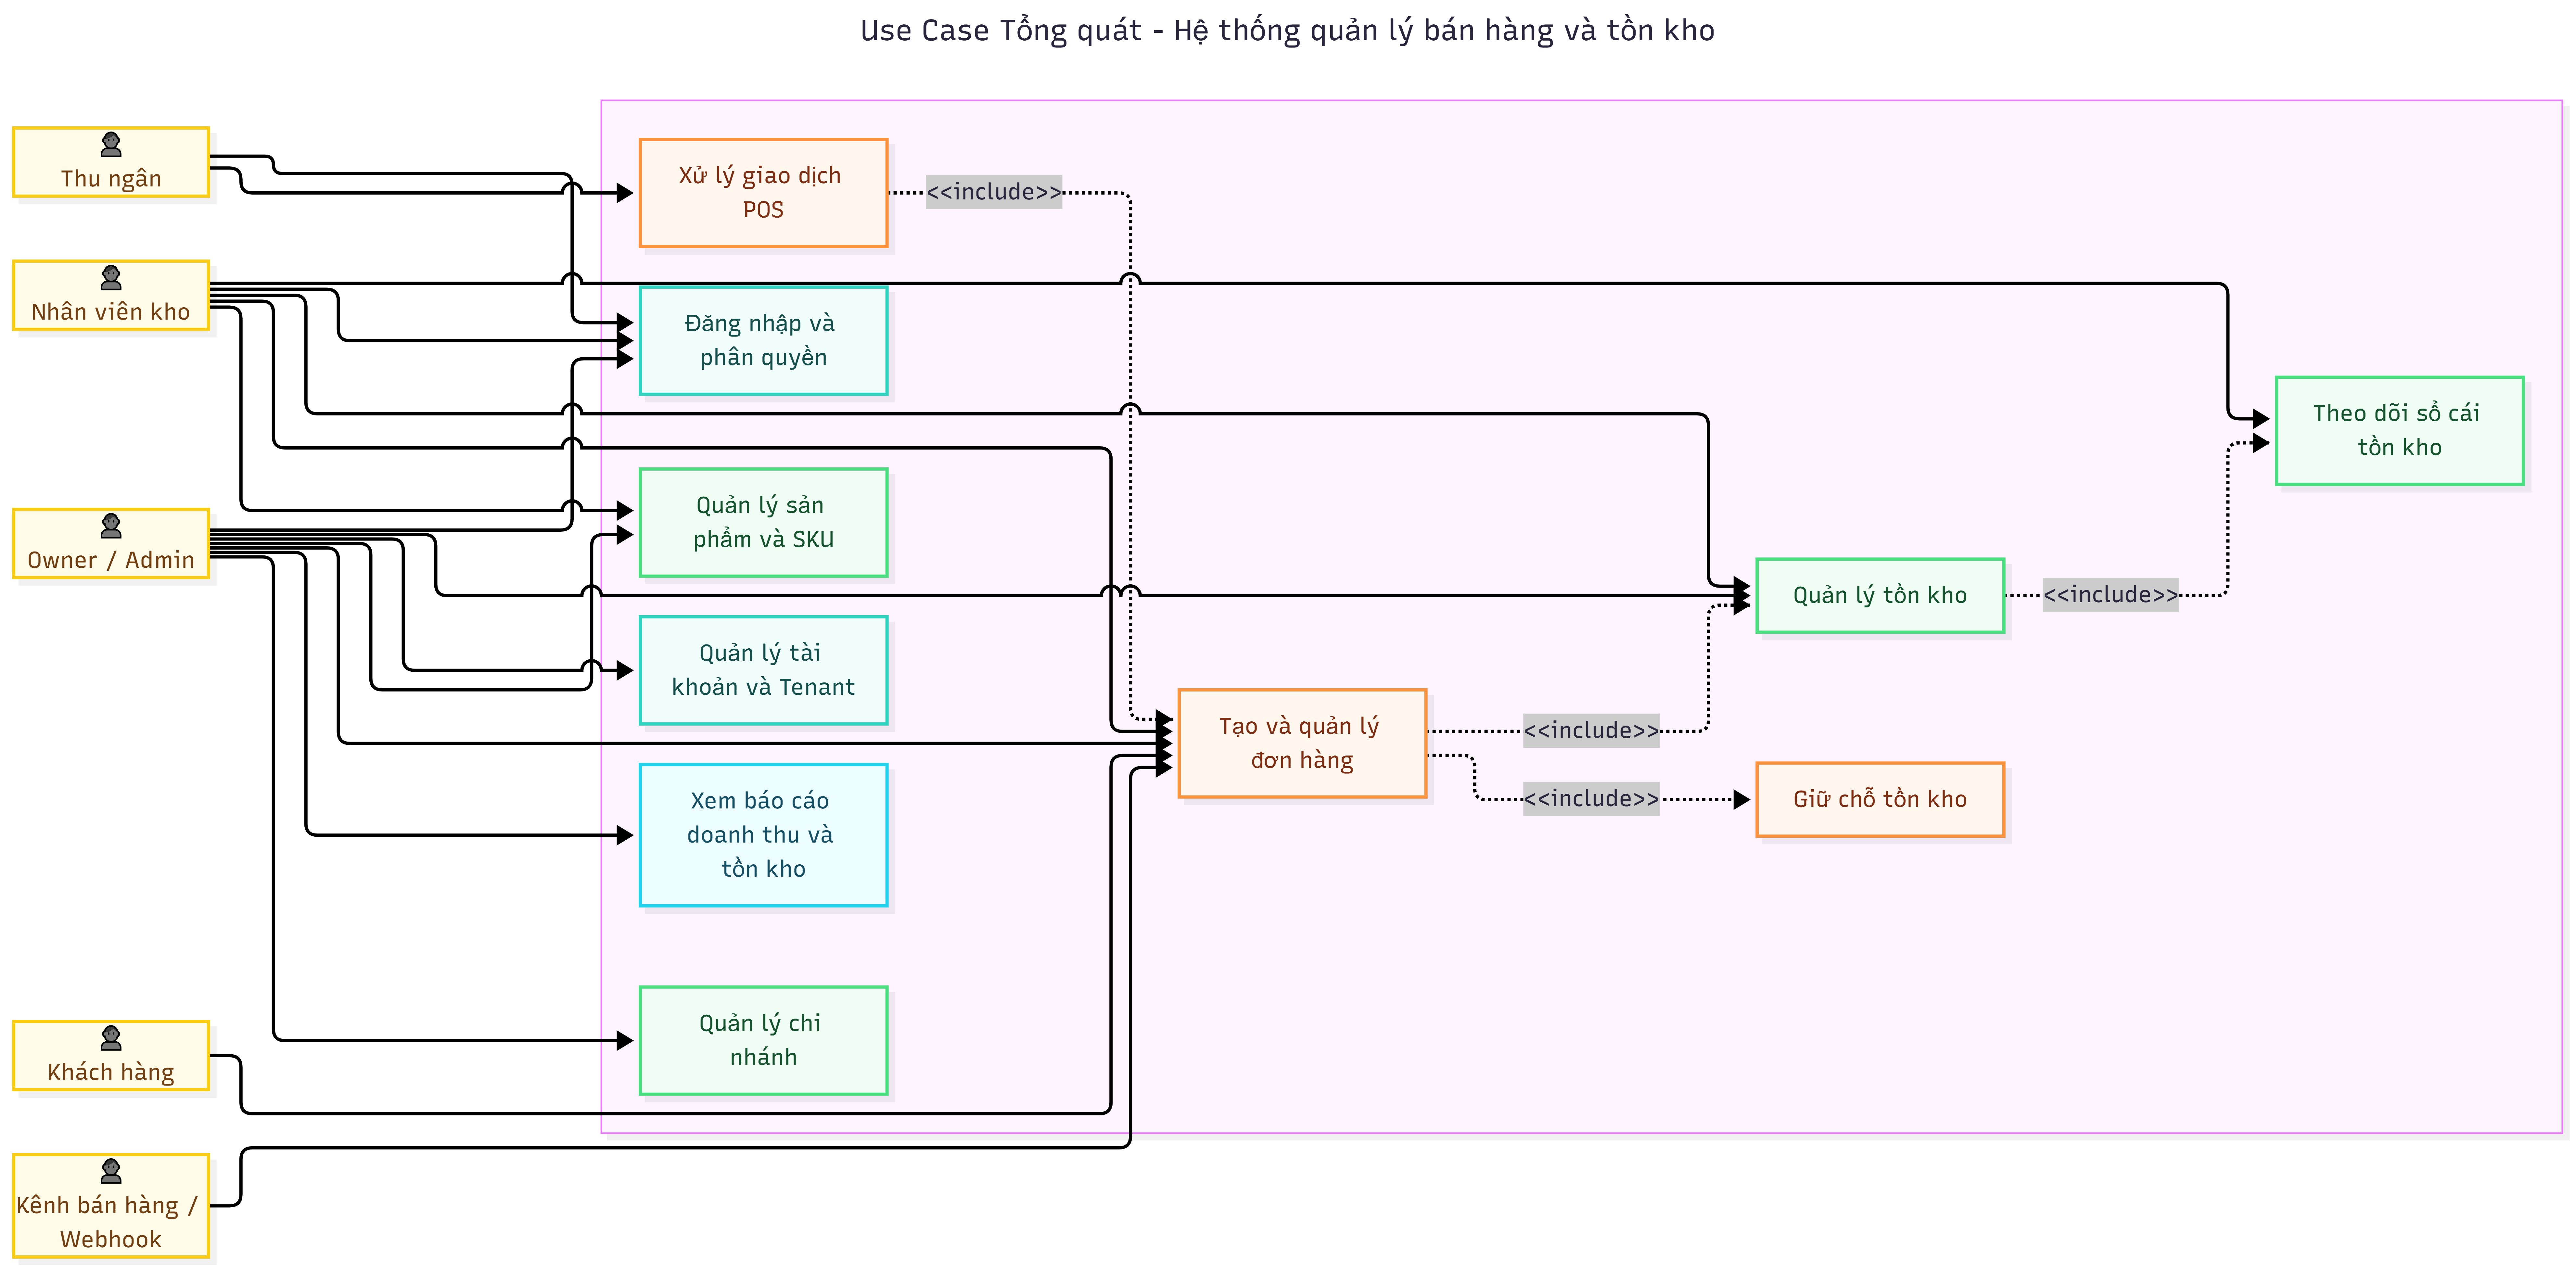
\includegraphics[width=0.88\textwidth]{Use case Tongquat.png}
		\caption{Sơ đồ Use Case tổng quát của hệ thống OISM}
	\end{figure}
	\begin{figure}[H]
		\centering
		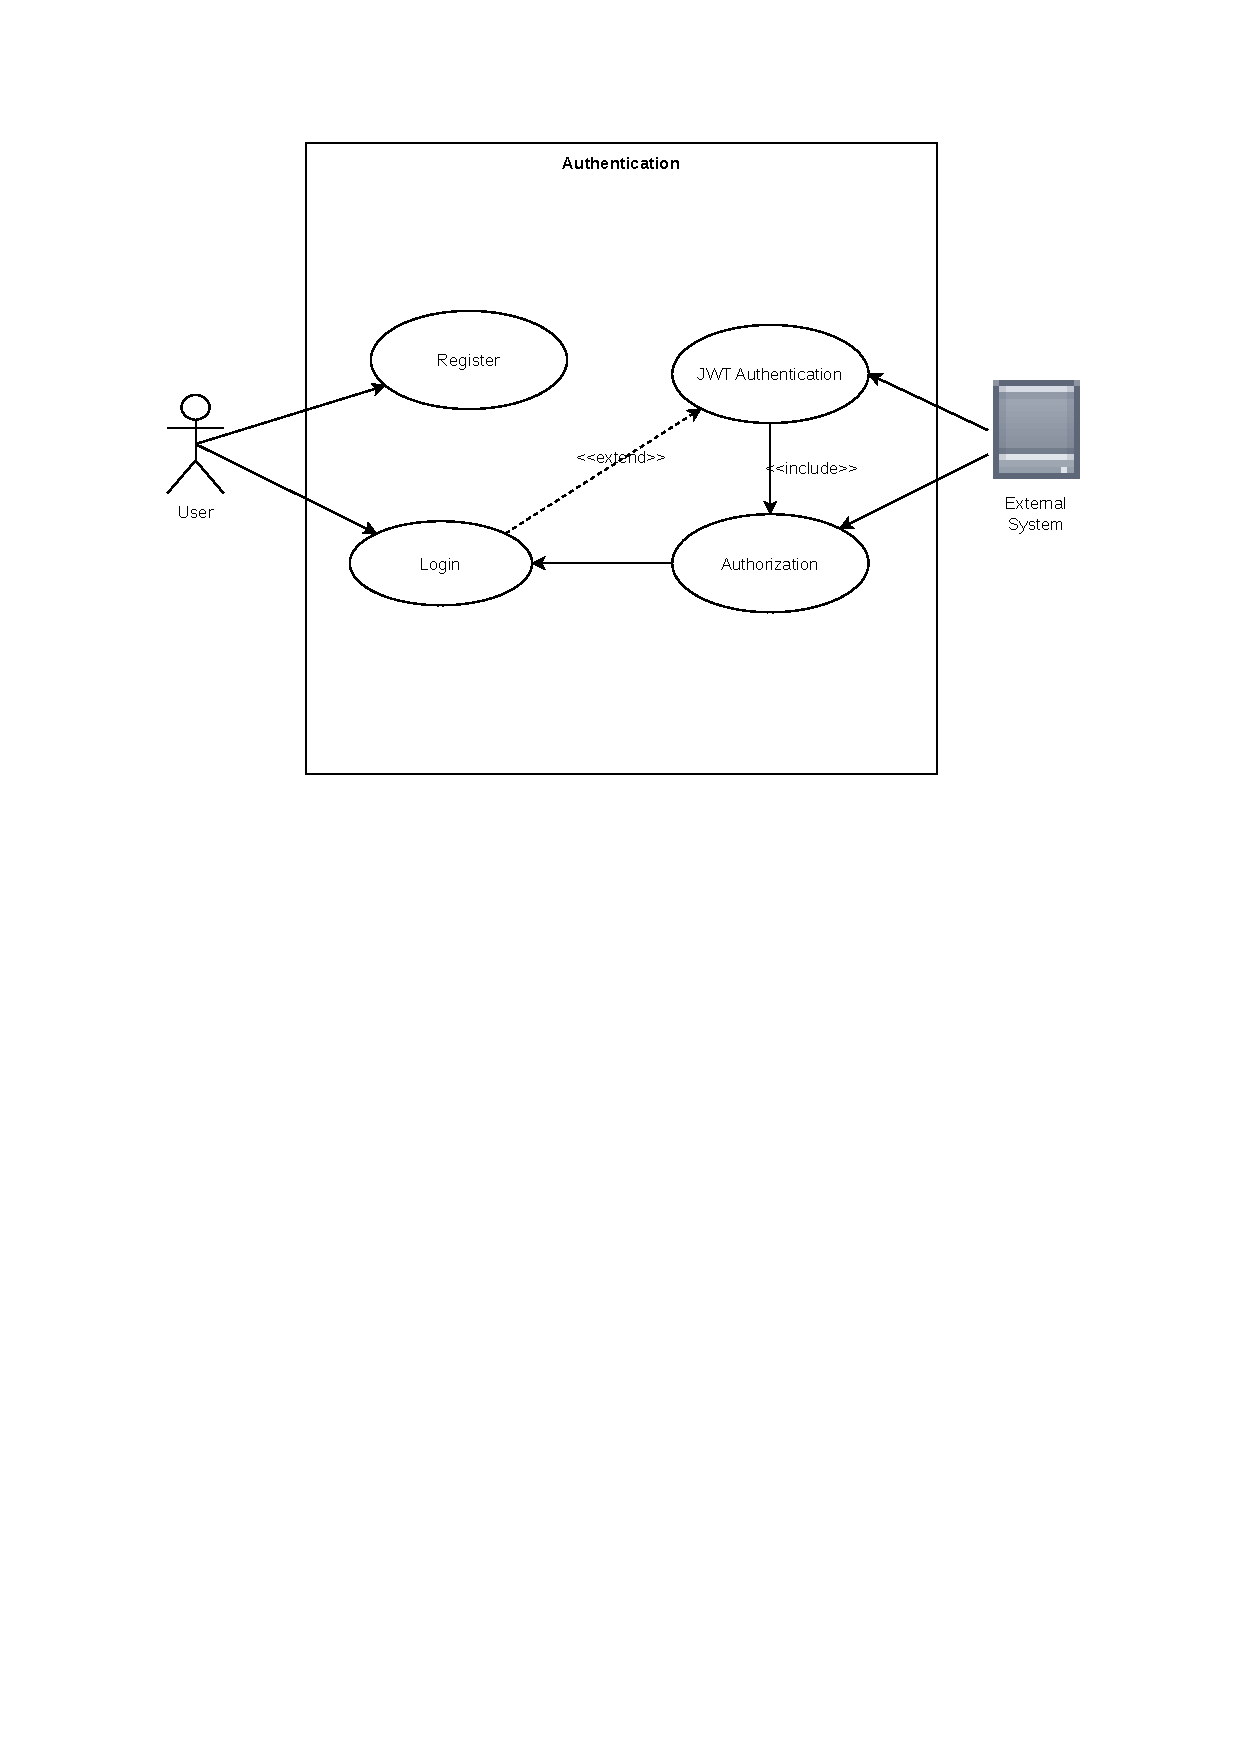
\includegraphics[width=0.88\textwidth]{Authentication.pdf}
		\caption{Sơ đồ Use Case phân hệ Xác thực}
	\end{figure}
	\begin{figure}[H]
		\centering
		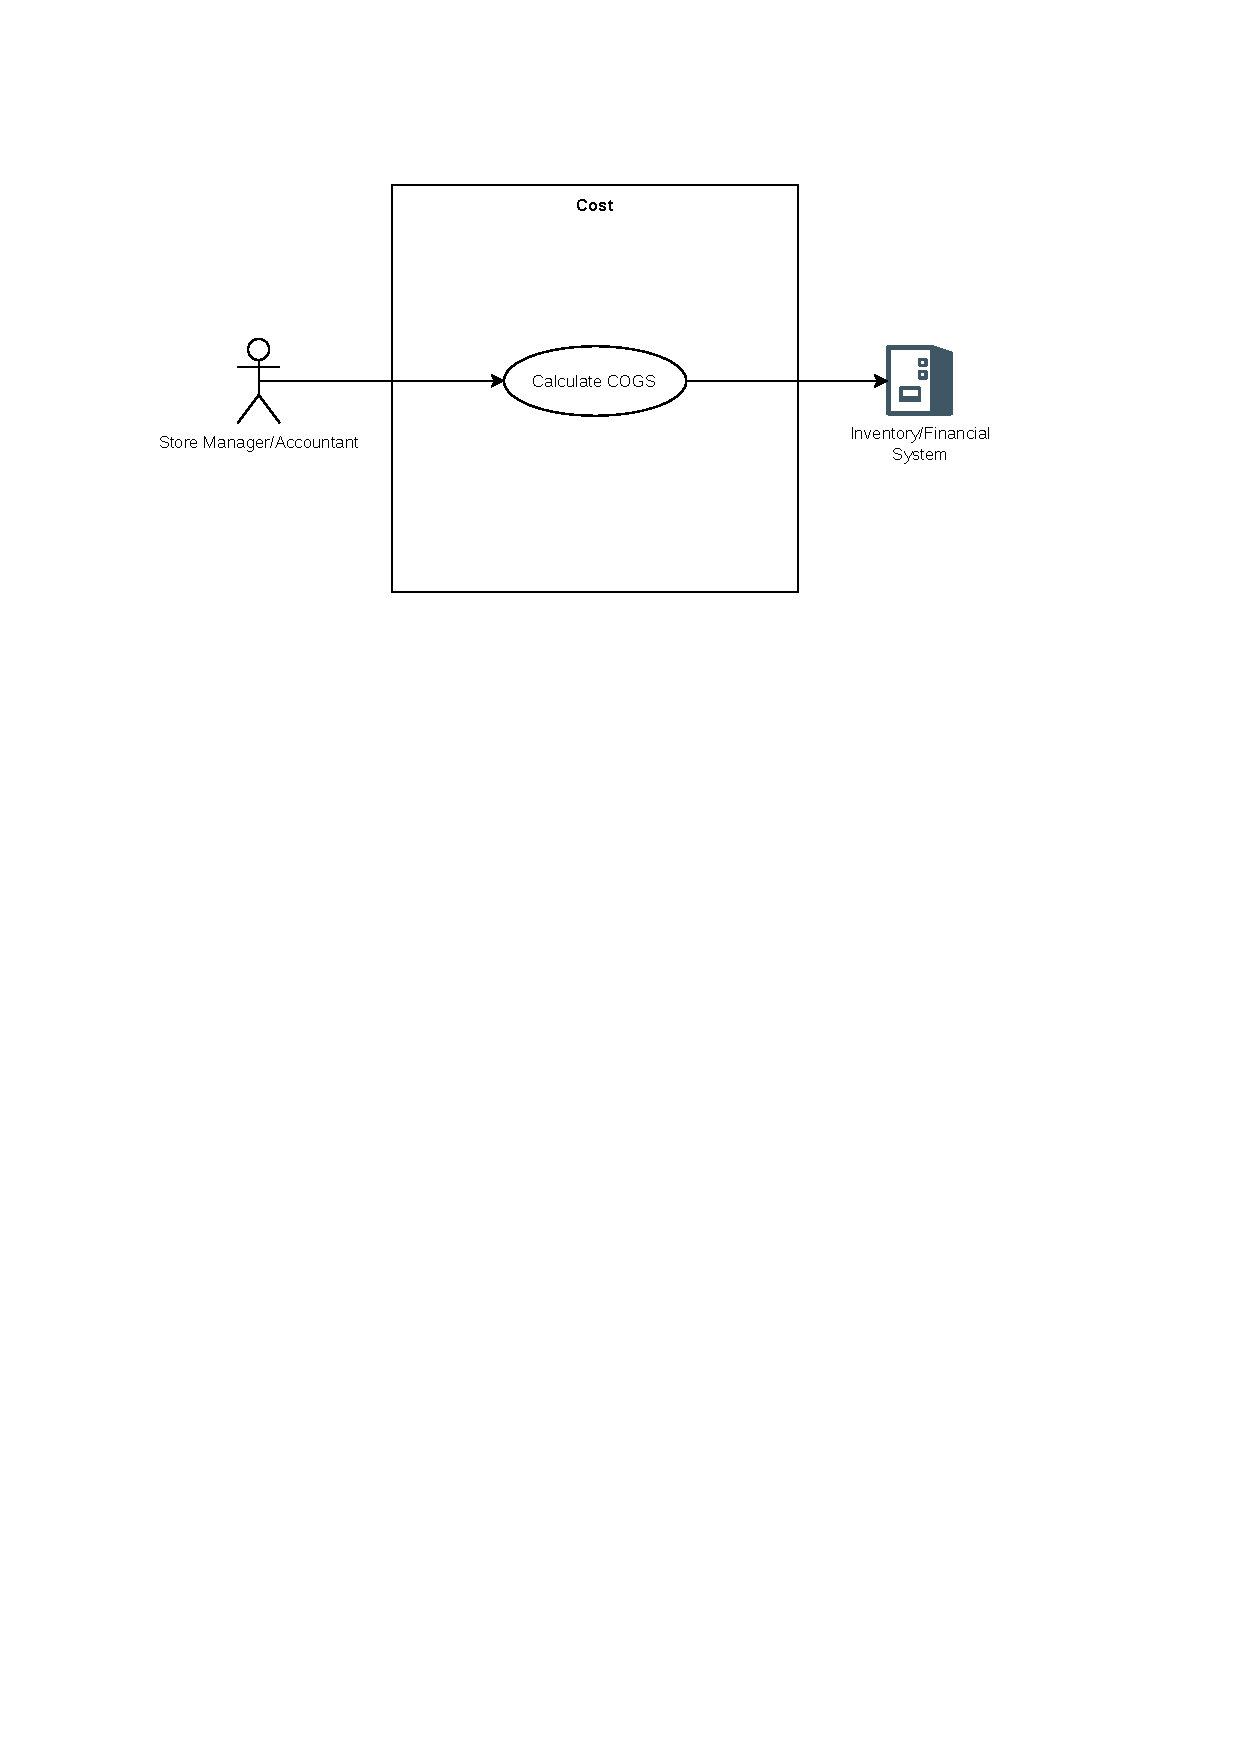
\includegraphics[width=0.88\textwidth]{Cost.pdf}
		\caption{Sơ đồ Use Case phân hệ Quản lý Chi phí \& Giá vốn}
	\end{figure}
	\begin{figure}[H]
		\centering
		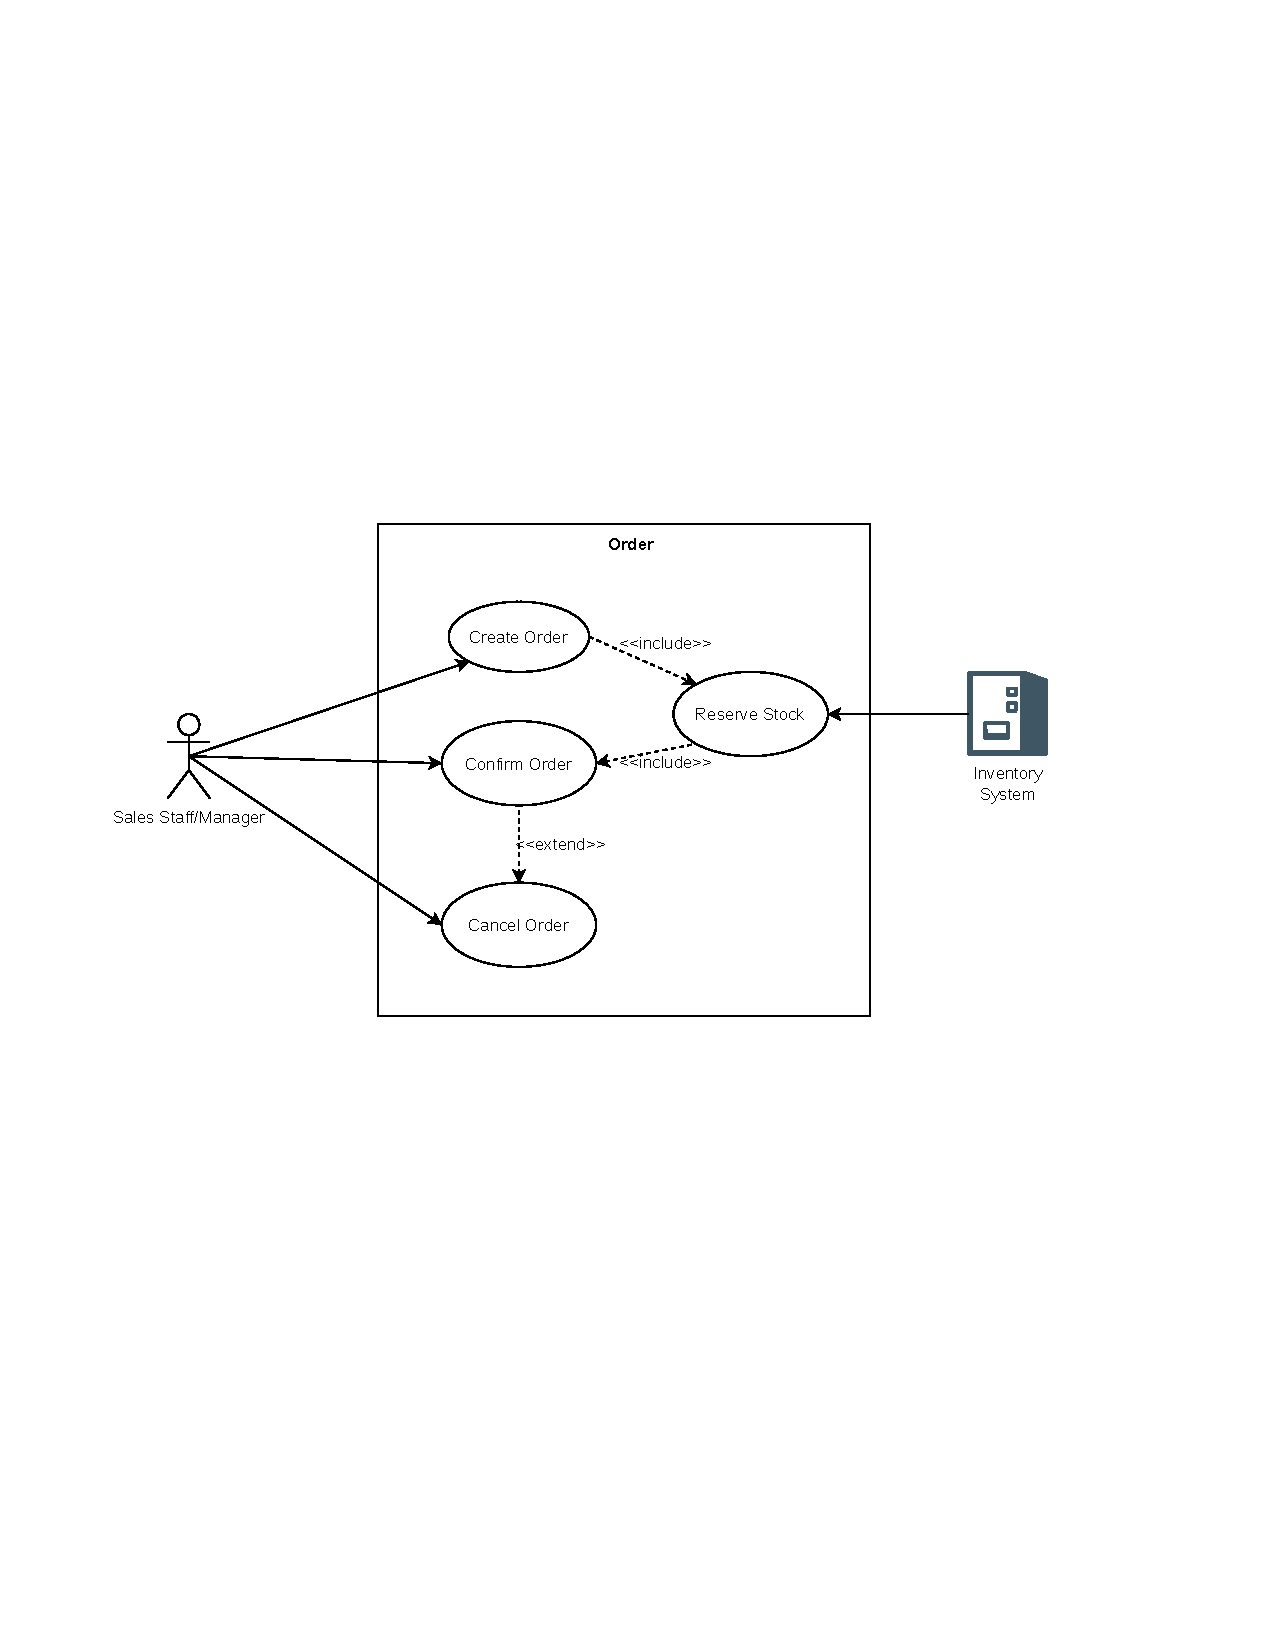
\includegraphics[width=0.88\textwidth]{Order.pdf}
		\caption{Sơ đồ Use Case phân hệ Đơn hàng}
	\end{figure}
	\begin{figure}[H]
		\centering
		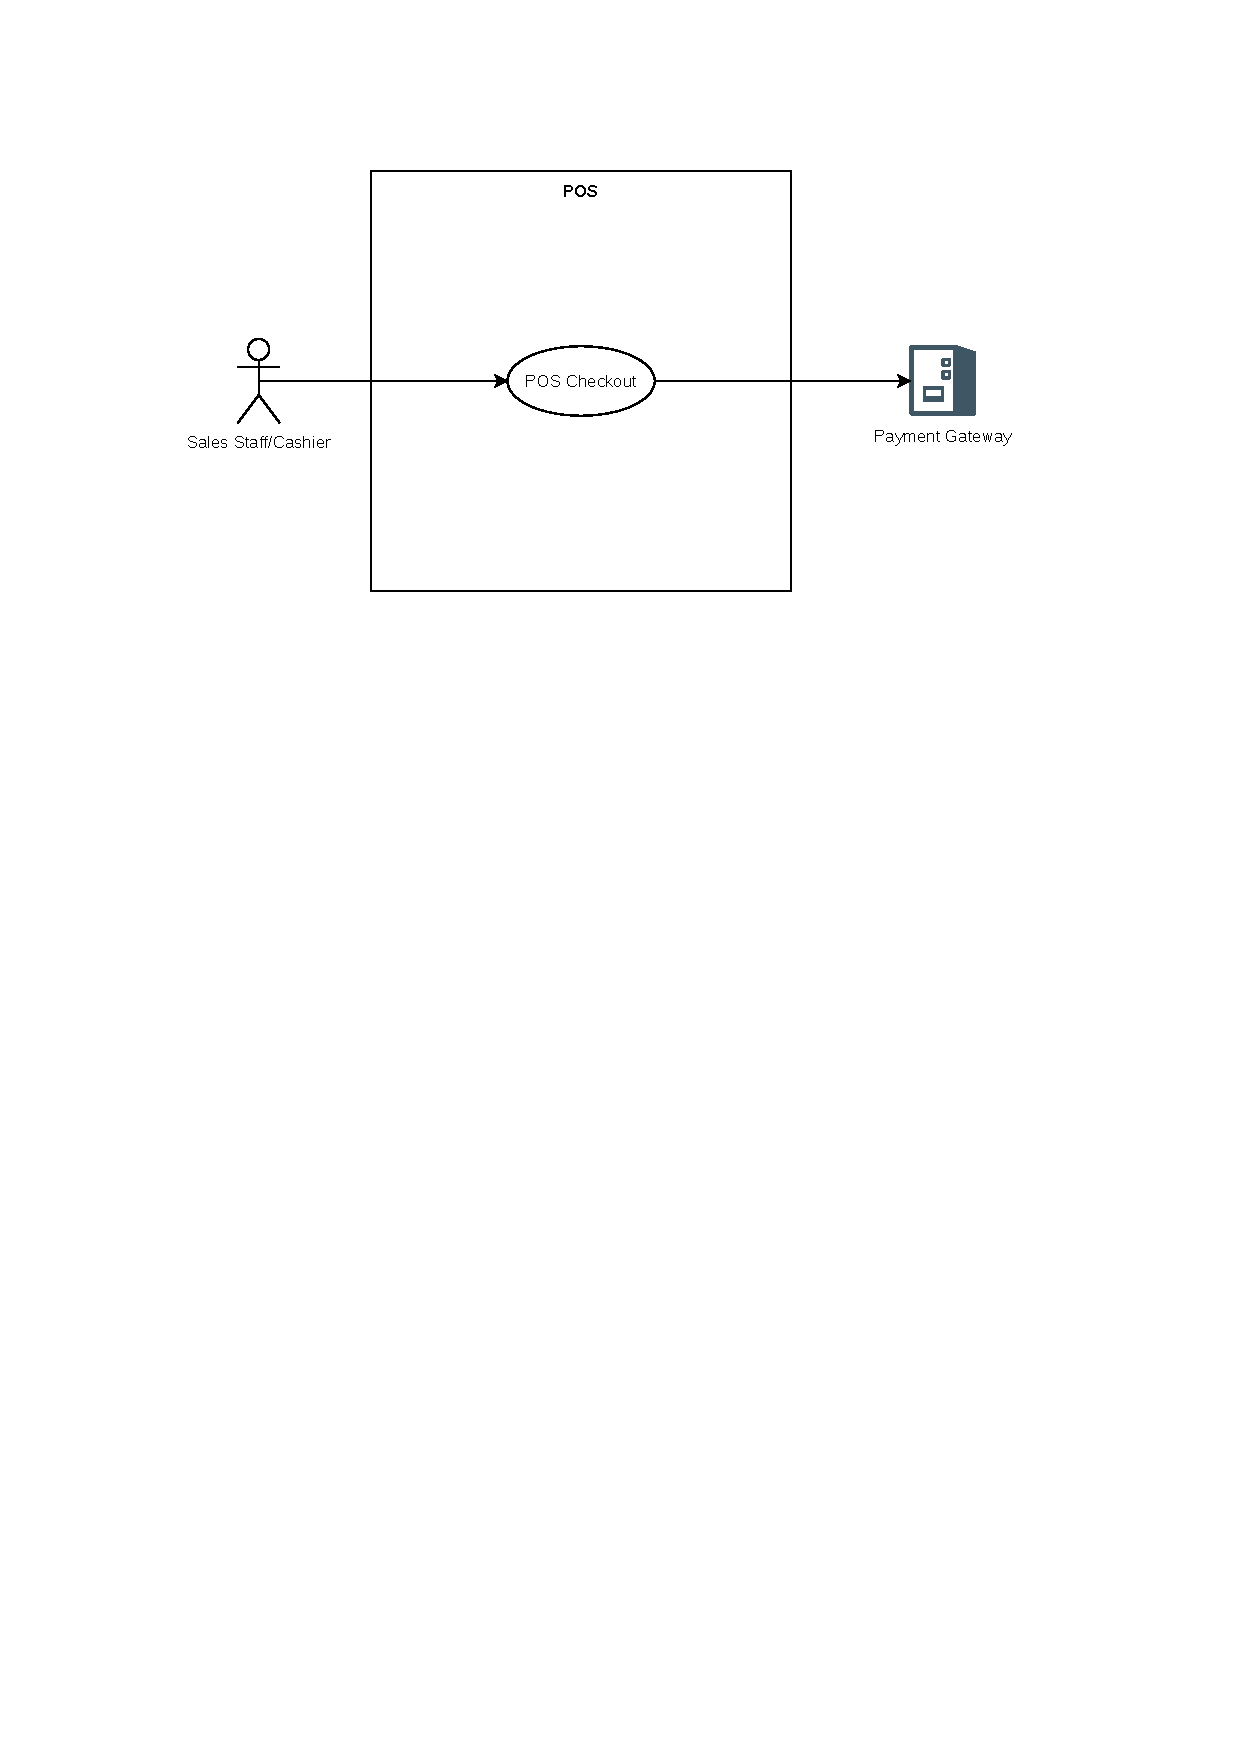
\includegraphics[width=0.88\textwidth]{POS.pdf}
		\caption{Sơ đồ Use Case phân hệ POS}
	\end{figure}
	\begin{figure}[H]
		\centering
		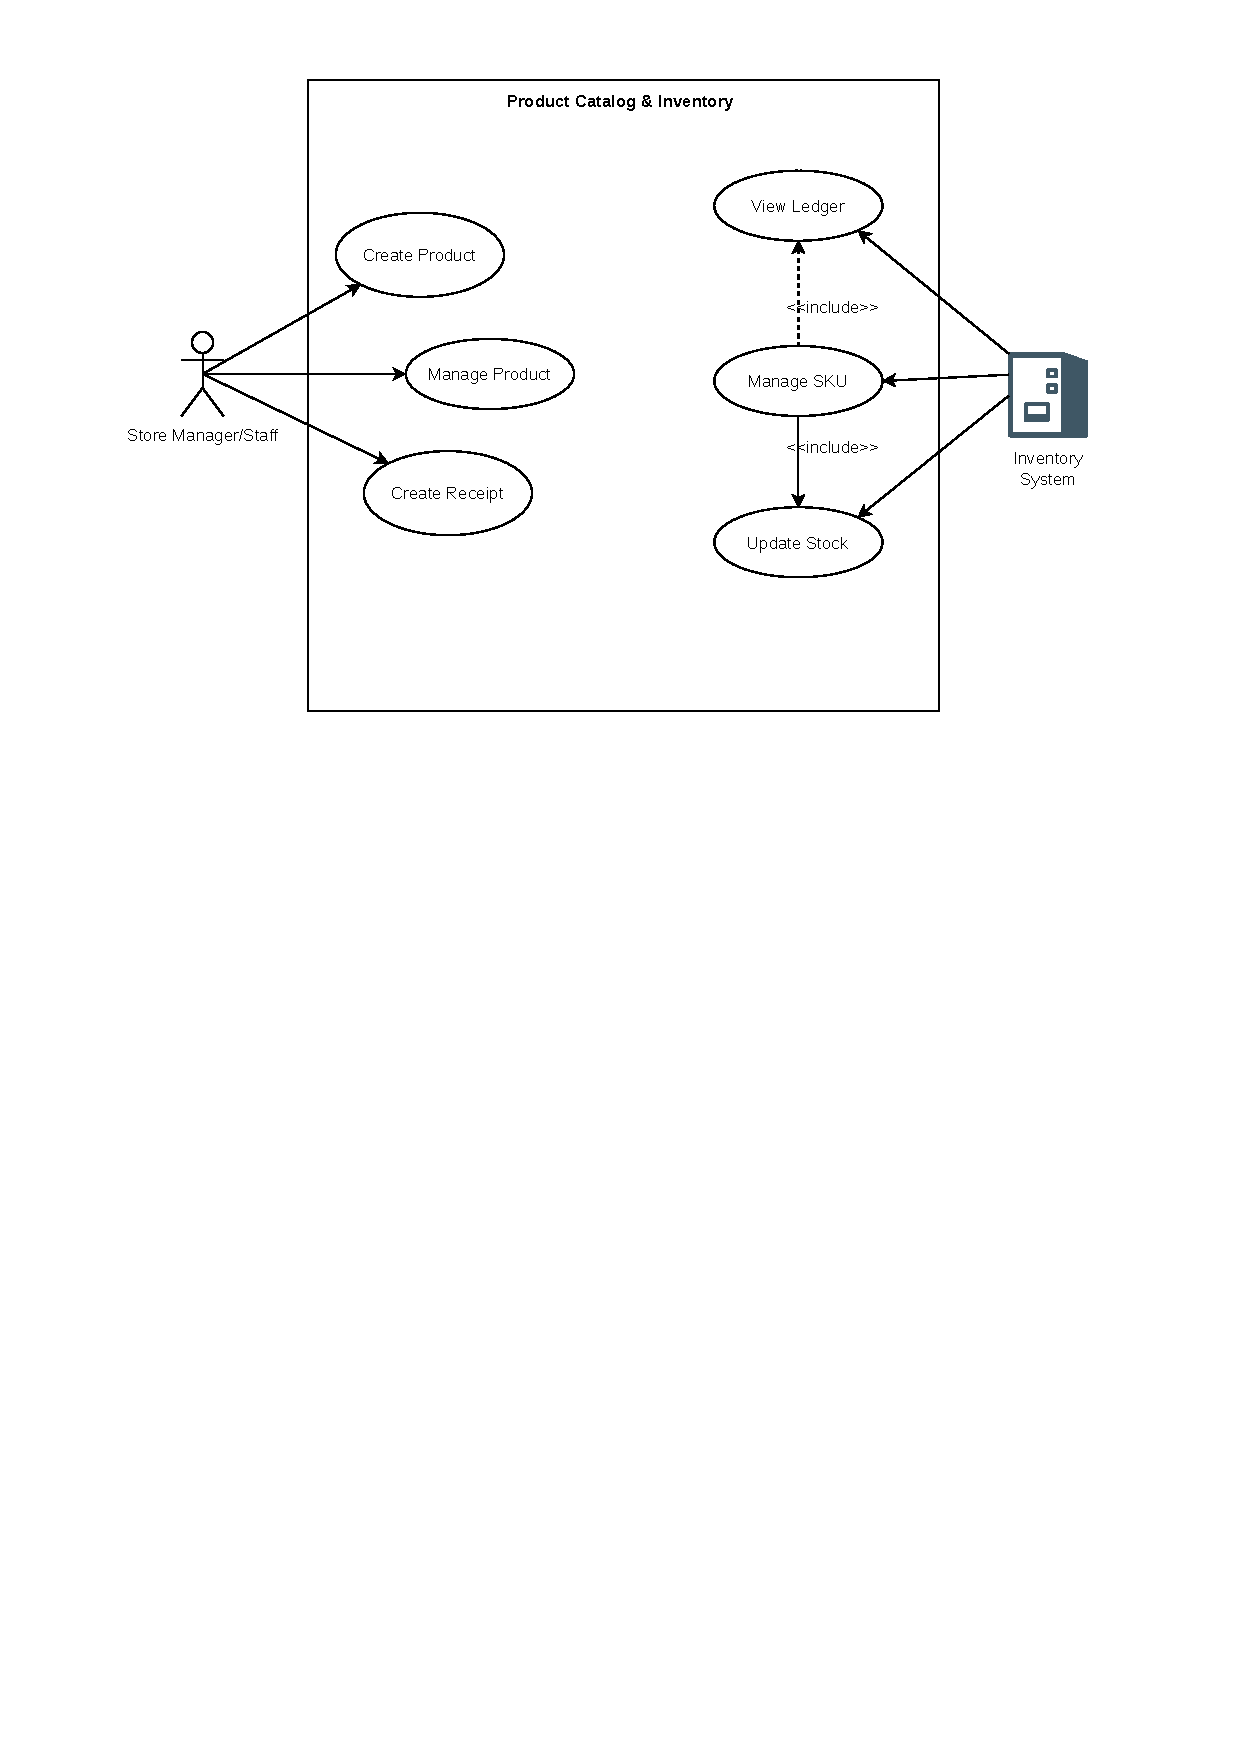
\includegraphics[width=0.88\textwidth]{Product Catalog & Inventory.pdf}
		\caption{Sơ đồ Use Case Quản lý Sản phẩm \& Tồn kho}
	\end{figure}
	\begin{figure}[H]
		\centering
		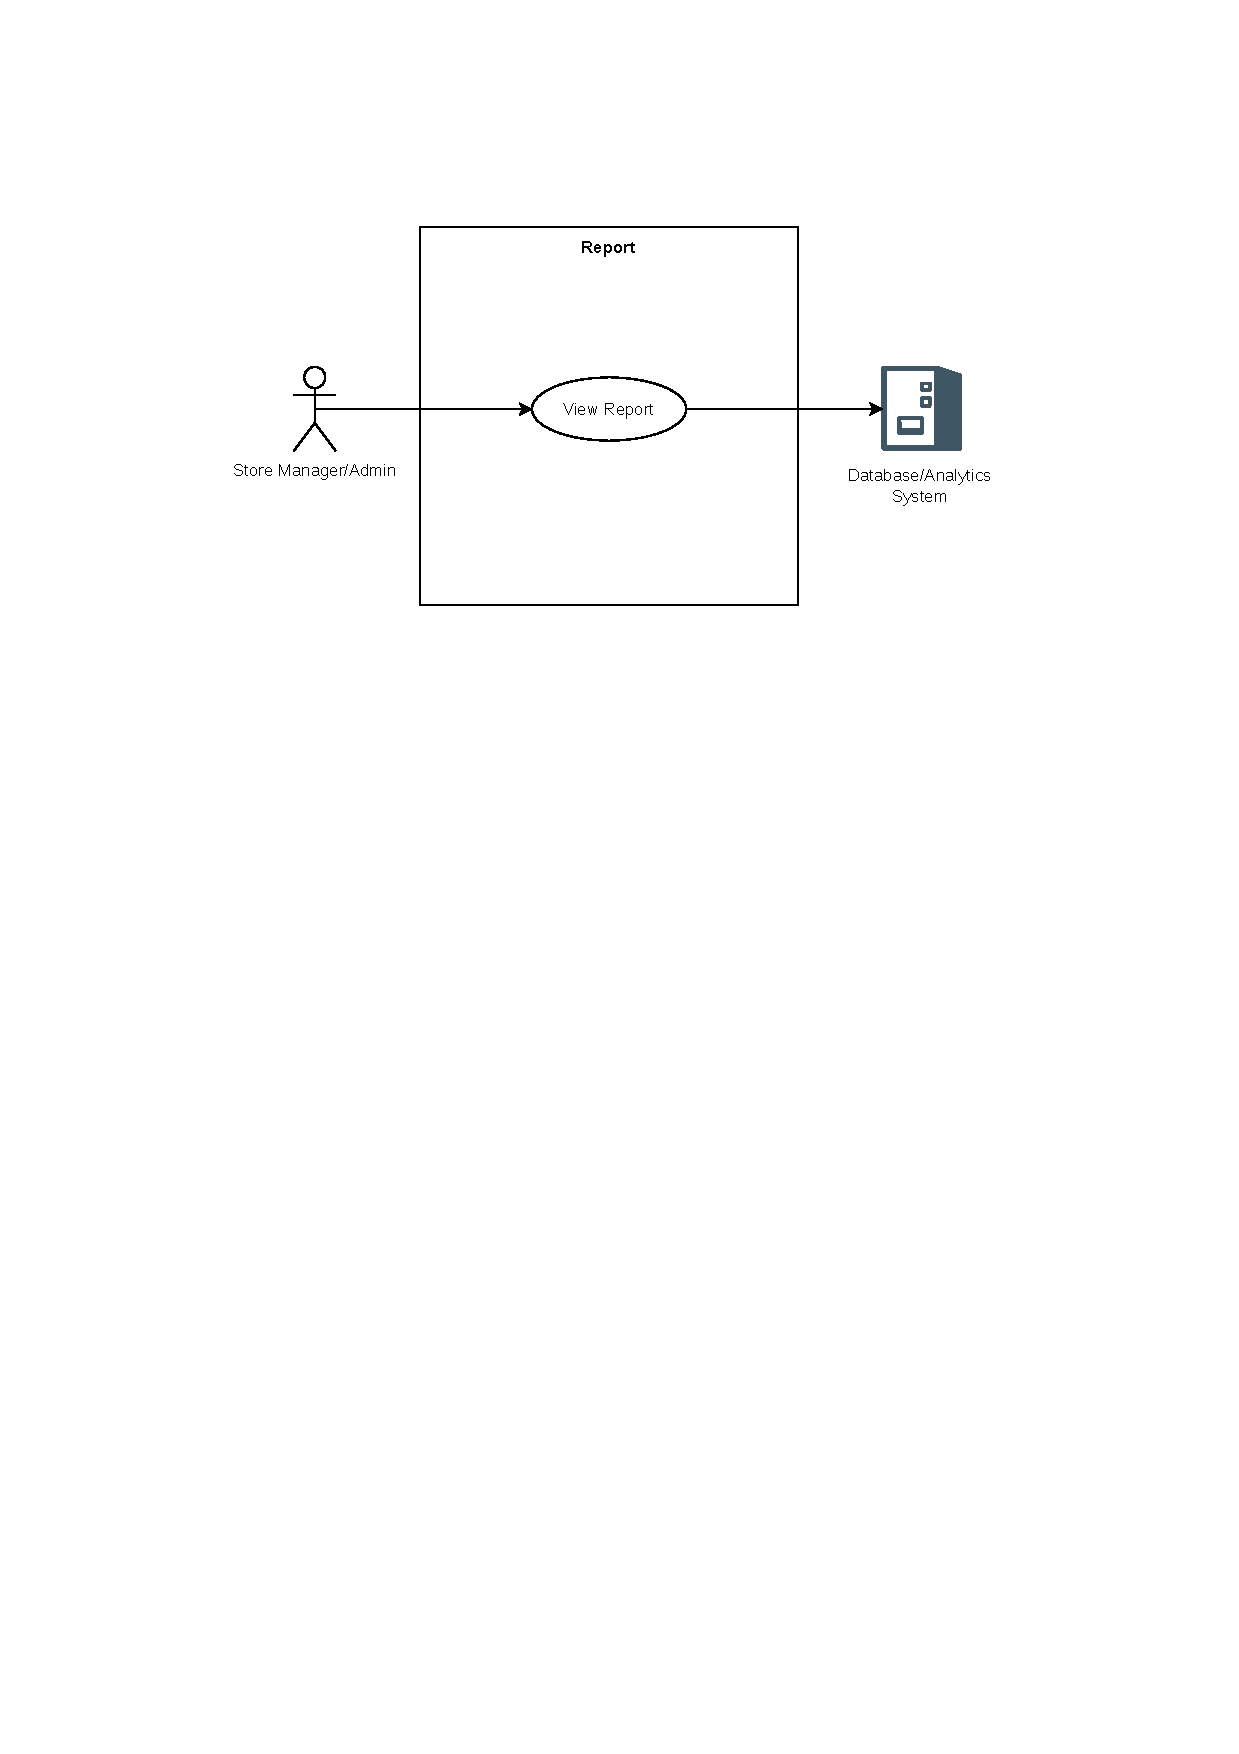
\includegraphics[width=0.88\textwidth]{Report.pdf}
		\caption{Sơ đồ Use Case phân hệ Báo cáo Thống kê}
	\end{figure}
	
	\section{Yêu cầu chức năng}
	Phân hệ yêu cầu chức năng đặc tả toàn bộ các tính năng cốt lõi mà hệ thống OISM phải cung cấp nhằm đáp ứng trọn vẹn nhu cầu quản lý bán lẻ đa kênh của doanh nghiệp. Các chức năng được phân rã cụ thể theo từng module như sau:
	\begin{itemize}
		\item \textbf{FR-AUTH (Quản lý Đa thuê bao và Xác thực):} Cung cấp tính năng đăng ký cửa hàng tenant với không gian dữ liệu độc lập, hỗ trợ xác thực người dùng qua Email/Điện thoại kèm mật khẩu để trả về mã thông báo JWT chứa định danh định tuyến; thực thi phân quyền RBAC chia rõ vai trò Owner, Staff và Cashier; đồng thời hỗ trợ chủ cửa hàng quản lý toàn bộ hệ thống chi nhánh trực thuộc.
		\item \textbf{FR-PROD (Quản lý Sản phẩm và Biến thể SKU):} Xây dựng danh mục phân cấp sản phẩm và thương hiệu, hỗ trợ sản phẩm đơn và sản phẩm có biến thể đa dạng (Màu sắc, Kích thước), tự động gán hoặc nhập thủ công mã vạch EAN-13/Code128 cho từng SKU, quản lý độc lập giá bán lẻ và giá sỉ.
		\item \textbf{FR-INV (Sổ cái Tồn kho và Quản lý Kho):} Ghi nhận nghiêm ngặt mọi biến động nhập, xuất, bán, trả hàng hay chuyển kho vào bảng sổ cái bất biến dạng chỉ-ghi-thêm (\textit{append-only ledger}) chứa đầy đủ thông tin định danh, số lượng và số dư còn lại; tuyệt đối cấm can thiệp cập nhật trực tiếp cột số lượng tồn thực tế. Đồng thời hỗ trợ quy trình nhập hàng từ nhà cung cấp và điều chuyển kho hai bước.
		\item \textbf{FR-COST (Tính toán Giá vốn Bình quân Gia quyền):} Tự động tính toán lại giá vốn đơn vị SKU ngay khi xác nhận phiếu nhập kho theo công thức gia quyền chính xác, đồng thời thực hiện chụp nhanh giá vốn vào chi tiết đơn hàng khi chuyển trạng thái xác nhận.
		\item \textbf{FR-ORD \& FR-RSE (Hub Đơn hàng và Chống bán quá tải):} Chuẩn hóa đơn hàng đa kênh về mô hình chuẩn, vận hành cỗ máy trạng thái vòng đời đơn hàng, đồng thời duy trì công thức tồn kho khả dụng để thực thi giữ chỗ tự động, vô hiệu hóa hoàn toàn hiện tượng bán vượt.
		\item \textbf{FR-POS, FR-REP \& FR-SIM (POS, Báo cáo và Mô phỏng):} Cung cấp giao diện PWA POS bán hàng siêu tốc hỗ trợ in hóa đơn qua trình duyệt, tổng hợp báo cáo doanh thu, lợi nhuận gộp, cùng công cụ giả lập webhook thương mại điện tử và xử lý thông báo thời gian thực qua SignalR.
	\end{itemize}
	
	\section{Yêu cầu phi chức năng}
	Bên cạnh các tính năng nghiệp vụ, hệ thống OISM đặt ra các tiêu chuẩn phi chức năng khắt khe nhằm đảm bảo chất lượng vận hành trong môi trường thực tế:
	\begin{itemize}
		\item \textbf{NFR-PERF (Hiệu năng và Xử lý đồng thời):} Độ trễ phản hồi API (p95) đối với các tác vụ tìm kiếm SKU hoặc quét mã vạch POS phải dưới 200ms; thời gian tạo đơn hàng dưới 500ms; đồng thời hệ thống phải chịu tải tốt trong các kịch bản Flash Sale nhờ cơ chế khóa dòng cơ sở dữ liệu.
		\item \textbf{NFR-TENANT (Đa thuê bao và Cô lập dữ liệu):} Đảm bảo an toàn tuyệt đối thông tin giữa các cửa hàng thông qua định danh trường \texttt{TenantId} trên mọi bảng dữ liệu kết hợp bộ lọc toàn cầu, tối ưu hóa chỉ mục Index để duy trì hiệu năng với hàng triệu bản ghi sổ cái.
		\item \textbf{NFR-SEC (Bảo mật và Toàn vẹn ACID):} Mật khẩu người dùng được băm an toàn qua thuật toán BCrypt; giao tiếp bảo mật qua TLS 1.3; mọi chuỗi giao dịch tạo đơn hàng và giữ chỗ bắt buộc thực hiện bên trong khối giao dịch nguyên tử ACID có khả năng rollback hoàn toàn khi xảy ra lỗi.
		\item \textbf{NFR-USA, MAINT (Khả năng sử dụng và Bảo trì):} Giao diện POS tối giản cho phép hoàn tất thanh toán dưới 3 cú click chuột; kiến trúc phần mềm tuân thủ nghiêm ngặt Clean Architecture, đảm bảo độ phủ kiểm thử tự động các module cốt lõi đạt tối thiểu 80\%.
	\end{itemize}
	
	\section{Quy tắc nghiệp vụ}
	Hệ thống vận hành dựa trên các quy tắc nghiệp vụ bất di bất dịch nhằm duy trì tính nhất quán xuyên suốt:
	\begin{itemize}
		\item Công thức tính tồn kho khả dụng luôn được duy trì ở trạng thái động: $\text{Available} = \text{OnHand} - \text{Reserved}$.
		\item Bảng sổ cái tồn kho (\textit{Inventory Ledger}) tuân thủ nguyên tắc bất biến (\textit{append-only}), tuyệt đối không cho phép thực hiện câu lệnh UPDATE hoặc DELETE trên dữ liệu cũ; mọi sai sót buộc phải điều chỉnh bằng bút toán bù trừ].
		\item Vòng đời đơn hàng phải tuân thủ nghiêm ngặt cỗ máy trạng thái: từ khởi tạo bản nháp (\textit{Draft}), chuyển sang giữ chỗ (\textit{Reserved}), xác nhận (\textit{Confirmed}) đến hoàn thành (\textit{Completed}) hoặc hủy bỏ (\textit{Cancelled}).
	\end{itemize}
	
	\section{Quy tắc kiểm tra dữ liệu}
	Nhằm ngăn chặn các sự cố nhập liệu sai lệch từ phía người dùng, hệ thống áp dụng các tiêu chuẩn kiểm tra dữ liệu khắt khe:
	\begin{itemize}
		\item Mọi trường thông tin bắt buộc (đánh dấu hoa thị trên giao diện) phải được kiểm tra tính hợp lệ đồng thời ở cả hai tầng Client-side và Server-side.
		\item Định dạng email, số điện thoại Việt Nam (10 chữ số bắt đầu bằng số 0), ngày tháng và tiền tệ VND phải tuân thủ đúng định dạng chuẩn.
		\item Mã SKU và mã vạch của sản phẩm phải đảm bảo tính duy nhất trong phạm vi của cùng một Tenant, không cho phép nhập các giá trị số lượng hoặc đơn giá có giá trị âm.
	\end{itemize}
	
	\section{Thông báo hệ thống}
	Hệ thống xây dựng danh mục mã thông báo phản hồi (Message Codes từ \texttt{MSG01} đến \texttt{MSG64}) nhằm chuẩn hóa toàn bộ các thông điệp hiển thị trên giao diện người dùng. Các thông báo lỗi, cảnh báo thành công hoặc thông tin hướng dẫn được thiết kế ngắn gọn, trực quan, không để lộ các ngoại lệ hệ thống hay stack trace kỹ thuật nhằm đảm bảo tính bảo mật và trải nghiệm chuyên nghiệp.
	
	\section{Ma trận truy vết yêu cầu}
	Ma trận truy vết yêu cầu (Requirement Traceability Matrix) được thiết lập nhằm tạo ra mối liên kết xuyên suốt và chặt chẽ giữa các yêu cầu chức năng của phần mềm với các module mã nguồn thực thi, các bảng dữ liệu liên quan và các kịch bản kiểm thử tương ứng[cite: 3]. Bảng ma trận này giúp đội ngũ phát triển dễ dàng kiểm soát tiến độ, đánh giá mức độ hoàn thành và phát hiện nhanh chóng các thiếu sót phát sinh trong suốt vòng đời phát triển dự án OISM.
	
	% ============================================================
	% CHƯƠNG 4. ĐẶC TẢ THIẾT KẾ PHẦN MỀM
	% ============================================================
	\chapter{ĐẶC TẢ THIẾT KẾ PHẦN MỀM}
	\section{Thiết kế kiến trúc hệ thống}
	Hệ thống áp dụng mô hình Client-Server phân tầng rõ rệt, giao tiếp thông qua giao thức RESTful API nhằm tách biệt hoàn toàn giữa logic giao diện và tầng xử lý nghiệp vụ trung tâm.
	
	\section{Clean Architecture}
	Áp dụng triệt để nguyên tắc Clean Architecture nhằm phân chia hệ thống thành các vòng tròn đồng tâm độc lập: Domain (chứa logic cốt lõi như thuật toán tính WAC, trạng thái đơn), Application (chứa các use-case nghiệp vụ), Infrastructure (giao tiếp CSDL PostgreSQL, Redis) và Presentation (Web API, POS PWA).
	
	\section{Thiết kế cơ sở dữ liệu}
	Sử dụng cơ sở dữ liệu quan hệ PostgreSQL với các ràng buộc khóa ngoại chặt chẽ, hỗ trợ giao dịch nguyên tử ACID và cơ chế khóa dòng đồng thời để duy trì tính nhất quán tuyệt đối của dữ liệu tồn kho.
	
	\section{Thiết kế ERD (Entity Relationship Diagram)}
	Sơ đồ thực thể mối quan hệ thể hiện cấu trúc liên kết toàn vẹn dữ liệu giữa các thực thể trọng tâm: \textbf{Tenants}, \textbf{Users}, \textbf{Branches}, \textbf{Products}, \textbf{SKUs}, \textbf{Inventory Transactions (Ledger)}, \textbf{Orders}, \textbf{OrderItems}, và \textbf{Reservations}.
	
	\begin{figure}[H]
		\centering
		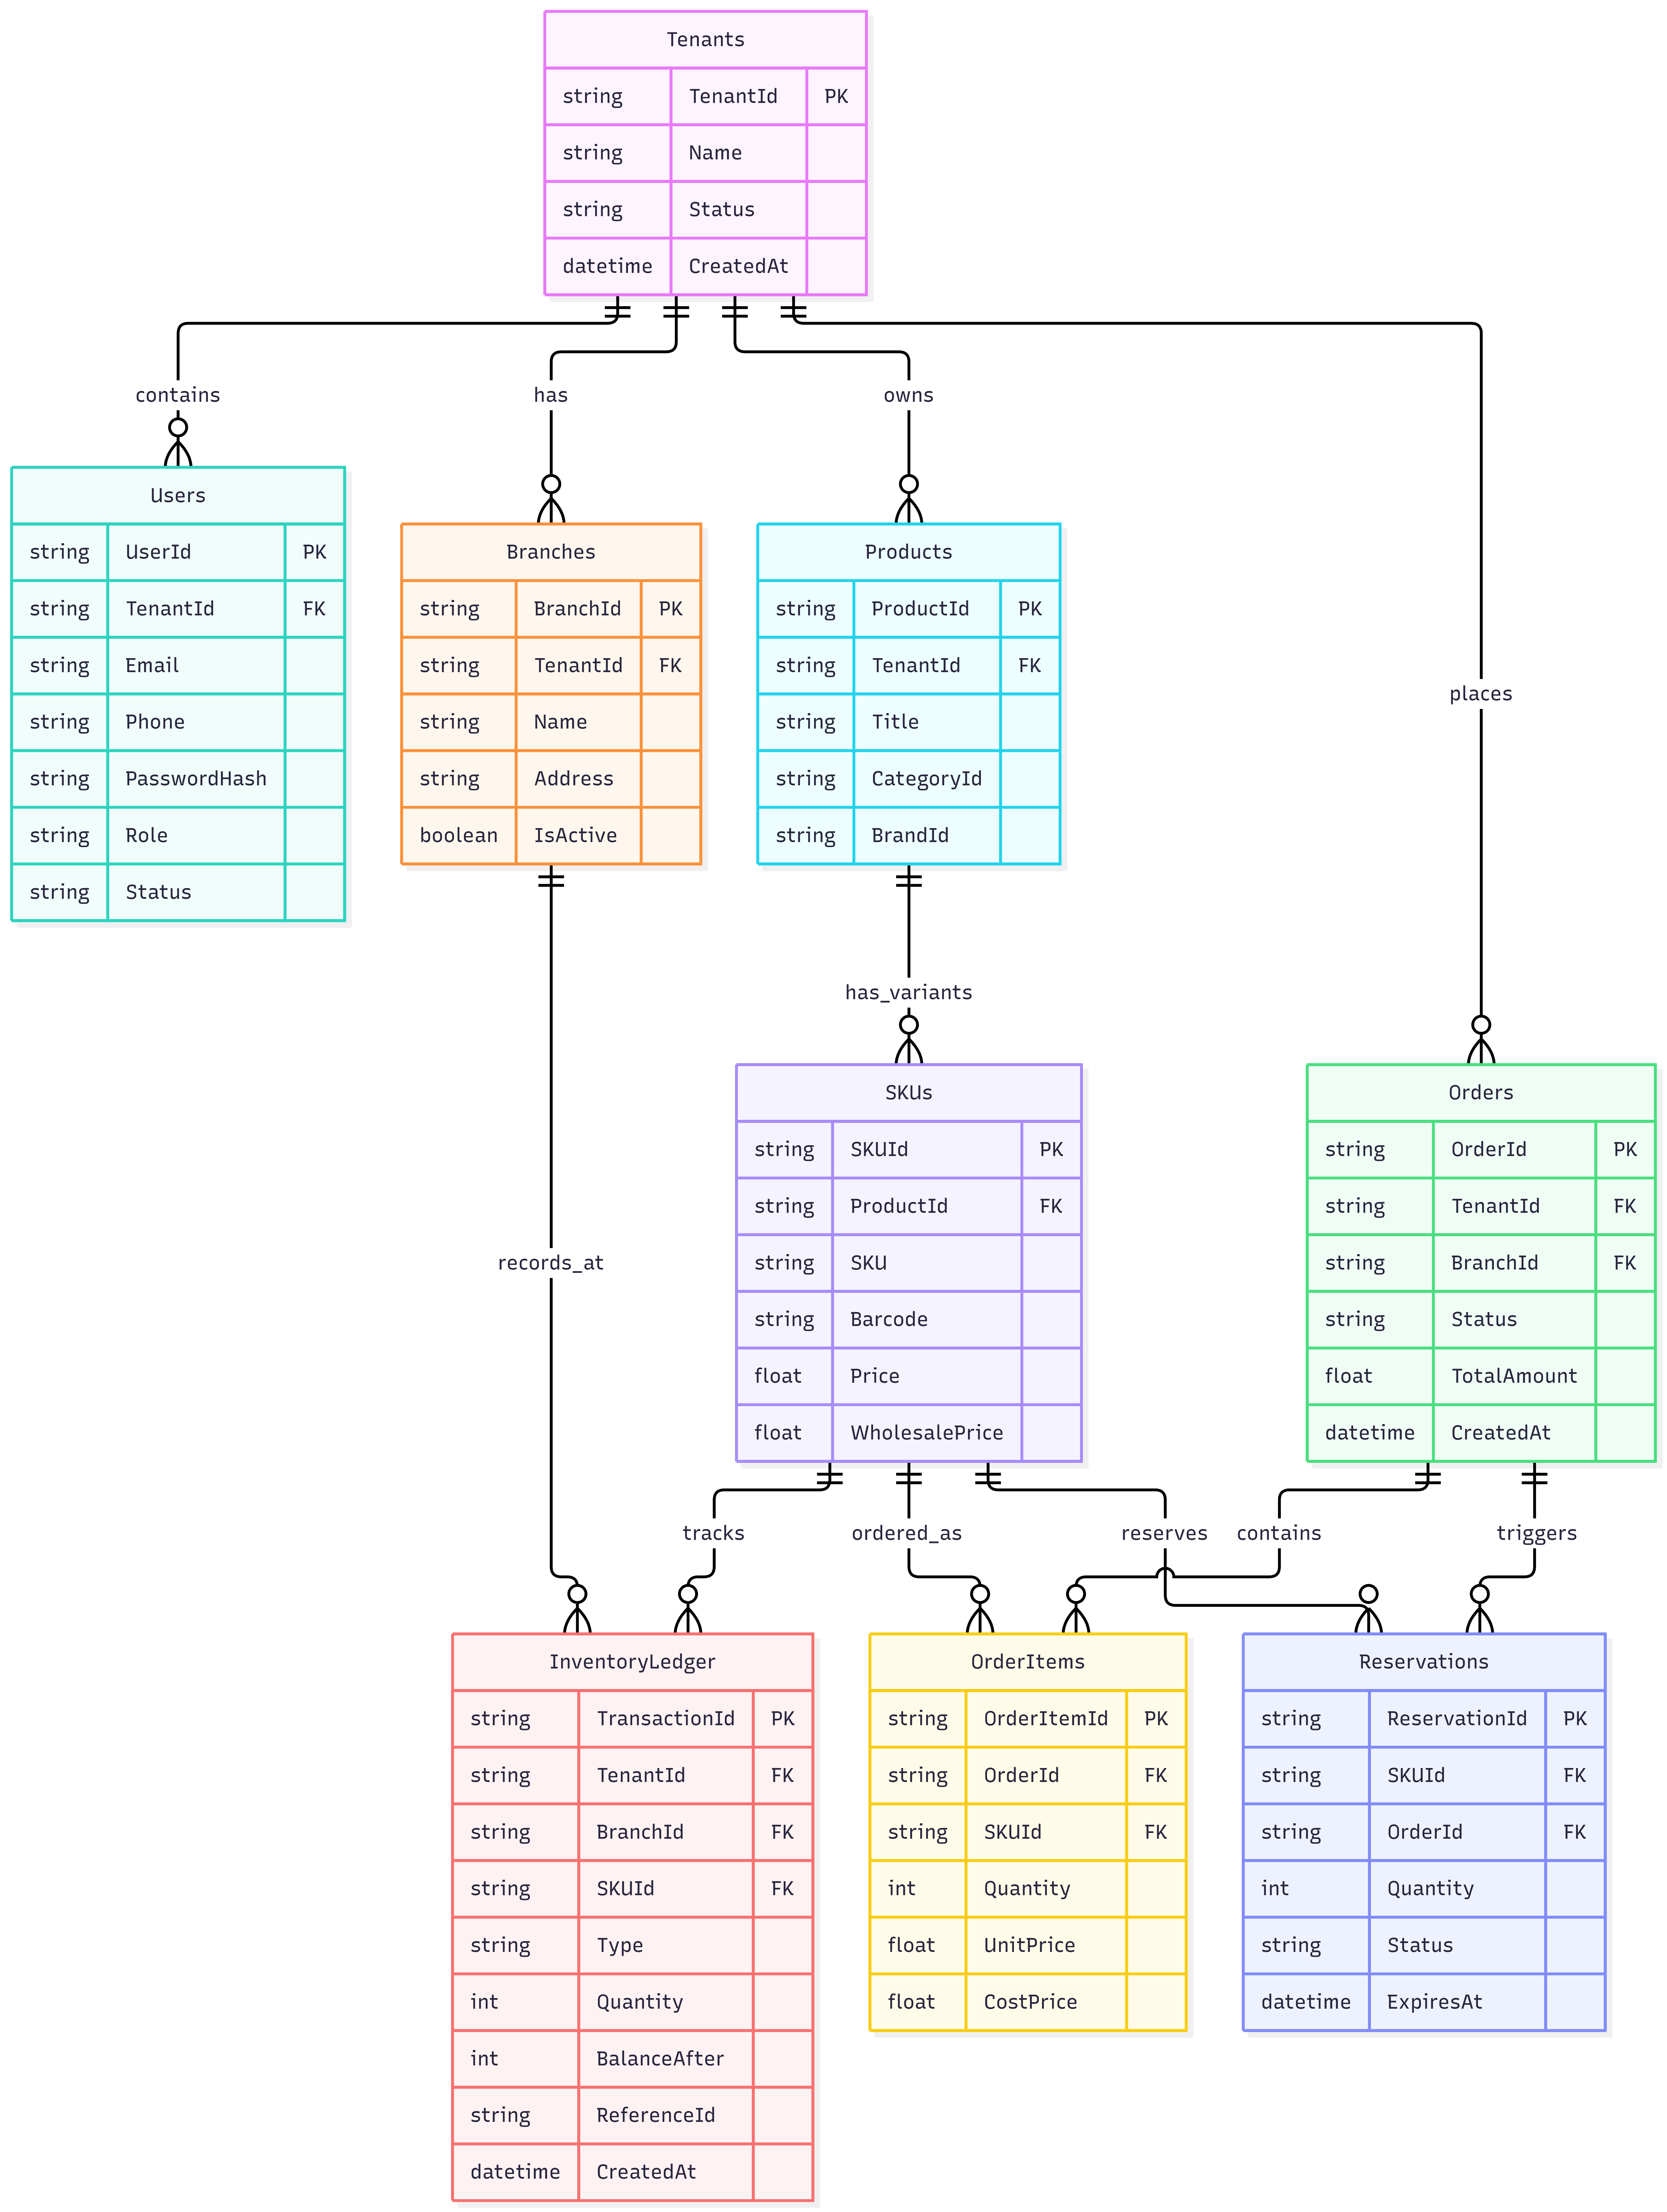
\includegraphics[width=0.88\textwidth]{ERD.png}
		\caption{Mô hình thực thể mối quan hệ (ERD) của hệ thống OISM}
	\end{figure}
	
	\section{Đặc tả các bảng}
	Trong cơ sở dữ liệu quan hệ PostgreSQL của hệ thống OISM, các bảng dữ liệu được thiết kế theo chuẩn hóa dạng chuẩn 3 (3NF) nhằm loại bỏ dị biệt, tối ưu không gian lưu trữ và đảm bảo tốc độ truy xuất. Dưới đây là đặc tả chi tiết các bảng dữ liệu cốt lõi:
	\par
	\begin{itemize}
		\item \textbf{Bảng Tenants:} đóng vai trò là thực thể gốc của mô hình SaaS đa thuê bao. Mỗi bản ghi đại diện cho một doanh nghiệp hoặc cửa hàng độc lập sử dụng hệ thống, được định danh bằng trường \texttt{TenantId} (Primary Key), kèm theo tên doanh nghiệp, trạng thái hoạt động và thời điểm khởi tạo hệ thống.
		\item \textbf{Bảng Users:} Quản lý toàn bộ thông tin định danh và bảo mật của người dùng trong hệ thống. Bảng này lưu trữ thông tin về email, số điện thoại, mật khẩu đã được băm an toàn qua thuật toán mật mã, liên kết trực tiếp với tenant tương ứng qua khóa ngoại \texttt{TenantId} và phân định quyền hạn thông qua trường vai trò \textit{Role}.
		\item \textbf{Bảng Branches:} Quản lý danh mục các chi nhánh cửa hàng và kho hàng trực thuộc quyền sở hữu của từng tenant, cho phép hệ thống phân tách rõ ràng lượng tồn kho vật lý giữa các điểm bán lẻ khác nhau.
		\item \textbf{Bảng Products \& SKUs:} Quản lý hệ thống phân cấp danh mục hàng hóa chung và các biến thể sản phẩm phân rã theo mã đơn vị lưu kho độc lập (\textit{SKU}). Mỗi SKU gắn liền với mã vạch (Barcode), giá bán lẻ, giá sỉ và liên kết trực tiếp với sản phẩm cha.
		\item \textbf{Inventory Ledger (Sổ cái tồn kho):} Bảng dữ liệu quan trọng nhất chịu trách nhiệm ghi nhận toàn bộ lịch sử biến động kho (Nhập hàng, Xuất bán, Trả hàng, Kiểm kê, Chuyển kho) theo nguyên tắc bất biến (\textit{Append-only}). Mọi dòng giao dịch đều ghi lại chi tiết loại giao dịch, số lượng thay đổi, số dư còn lại sau giao dịch (\textit{BalanceAfter}) và tham chiếu mã chứng từ gốc, tuyệt đối không cho phép thao tác sửa đổi hay xóa bỏ dữ liệu cũ.
		\item \textbf{Orders \& OrderItems:} Hub tập trung lưu trữ thông tin các đơn hàng đa kênh. Bảng đơn hàng quản lý trạng thái vòng đời (\textit{Draft, Reserved, Confirmed, Completed, Cancelled}), trong khi bảng chi tiết đơn hàng lưu trữ danh sách các mặt hàng SKU kèm theo đơn giá và giá vốn hàng bán (\textit{COGS}) được chụp nhanh tại thời điểm xác nhận.
	\end{itemize}
	
	\section{Thiết kế chỉ mục}
	Khi hệ thống vận hành thực tế trong môi trường doanh nghiệp, lượng bản ghi phát sinh trong các bảng giao dịch kho (\textit{Inventory Ledger}) và bảng đơn hàng (\textit{Orders}) có thể lên đến hàng triệu dòng chỉ sau một thời gian ngắn. Nếu không có chiến lược tối ưu hóa truy vấn, hiệu năng của toàn bộ hệ thống sẽ suy giảm nghiêm trọng.
	\par
	Để giải quyết bài toán này, hệ thống áp dụng chiến lược thiết kế chỉ mục (Indexing) nâng cao. Bên cạnh các khóa chính được tự động tạo Index, kiến trúc cơ sở dữ liệu thiết lập các Composite Index (Chỉ mục kết hợp) quan trọng bao gồm:
	\begin{itemize}
		\item \textbf{Index trên Inventory Ledger:} Thiết lập trên cặp trường \texttt{(TenantId, SKUId)} và \texttt{(TenantId, CreatedAt)} nhằm tăng tốc độ truy xuất lịch sử giao dịch kho, phục vụ tính toán tồn kho theo thời gian thực và trích xuất báo cáo nhanh chóng mà không phải quét toàn bộ bảng (\textit{Full Table Scan}).
		\item \textbf{Index trên Orders:} Thiết lập trên cặp trường \texttt{(TenantId, Status)} và \texttt{(TenantId, CreatedAt)} giúp tối ưu hóa các câu lệnh truy vấn lọc đơn hàng theo trạng thái chờ xử lý hoặc theo khoảng thời gian trên giao diện quản trị Admin Dashboard.
	\end{itemize}
	
	\section{Thiết kế Multi-tenancy}
	Mô hình SaaS đa thuê bao (Multi-tenant Architecture) được lựa chọn nhằm tối ưu hóa chi phí hạ tầng phần cứng, cho phép nhiều doanh nghiệp khách hàng cùng sử dụng một hệ thống phần mềm duy nhất nhưng vẫn đảm bảo sự cách ly thông tin chặt chẽ ở cấp độ logic.
	\par
	\begin{itemize}
		\item \textbf{Cô lập dữ liệu cấp độ ứng dụng:} Toàn bộ các bảng dữ liệu nghiệp vụ trong cơ sở dữ liệu PostgreSQL đều bắt buộc phải chứa trường khóa ngoại định danh \texttt{TenantId}. Mọi câu lệnh truy vấn dữ liệu phát sinh từ tầng ứng dụng đều phải tuân thủ việc truyền tham số \texttt{TenantId} tương ứng với phiên làm việc của người dùng hiện tại.
		\item \textbf{Global Query Filters (Bộ lọc toàn cầu):} Tận dụng sức mạnh của tầng ORM (Entity Framework Core / SQLAlchemy), hệ thống thiết lập bộ lọc truy vấn toàn cầu tự động đính kèm mệnh đề \texttt{WHERE TenantId = ?} vào mọi câu lệnh SQL truy xuất dữ liệu, giúp lập trình viên hoàn toàn tránh được rủi ro quên lọc dữ liệu giữa các tenant và triệt tiêu nguy cơ rò rỉ thông tin nhạy cảm.
	\end{itemize}
	
	\section{Thiết kế chi tiết các thành phần}
	Phần này trình bày cấu trúc chi tiết của các lớp đối tượng, các đối tượng truyền tải dữ liệu (Data Transfer Objects - DTOs) và các thành phần giao tiếp cấu thành nên hệ thống.
	\par
	Quá trình thiết kế chi tiết tuân thủ nguyên tắc đóng gói cao và lỏng lẻo về liên kết (\textit{Low Coupling, High Cohesion}). Cụ thể, các yêu cầu từ phía giao diện người dùng (Presentation Layer) sẽ được đóng gói vào các lớp Request DTO, sau đó được kiểm tra tính hợp lệ bằng các cơ chế xác thực tự động trước khi chuyển giao cho tầng dịch vụ xử lý nghiệp vụ (Business Service Layer). Tại đây, các quy tắc miền (Domain Rules) như tính toán giá vốn bình quân gia quyền hoặc kiểm tra tồn kho khả dụng được thực thi, sau đó kết quả được ánh xạ (Mapping) ngược lại thông qua các lớp Response DTO để trả về cho người dùng dưới định dạng chuẩn JSON qua RESTful API.
	
	\section{Class Diagram}
	Biểu đồ lớp (Class Diagram) mô tả cấu trúc tĩnh của hệ thống OISM, thể hiện rõ các lớp đối tượng, các thuộc tính, các phương thức hành vi và mối quan hệ tương quan (kết hợp, phụ thuộc, kế thừa) giữa các thành phần trong mã nguồn.
	\par
	Trong sơ đồ lớp của hệ thống, các đối tượng được phân rã theo đúng tinh thần của Clean Architecture. Các lớp thực thể miền (\textit{Domain Entities}) nằm ở tâm điểm, chứa đựng các thuộc tính nghiệp vụ thuần túy và không phụ thuộc vào bất kỳ công nghệ lưu trữ ngoài nào. Bao quanh chúng là các lớp Dịch vụ ứng dụng (\textit{Application Services}) chịu trách nhiệm điều phối luồng thực thi, các lớp Repository đóng vai trò trừu tượng hóa tầng truy xuất cơ sở dữ liệu, và các lớp Controller tiếp nhận yêu cầu HTTP từ phía client. Mô hình này giúp mã nguồn trở nên dễ đọc, dễ mở rộng và cực kỳ thuận lợi cho việc viết các kịch bản kiểm thử độc lập.
	
	\section{Sequence Diagram}
	\begin{figure}[H]
		\centering
		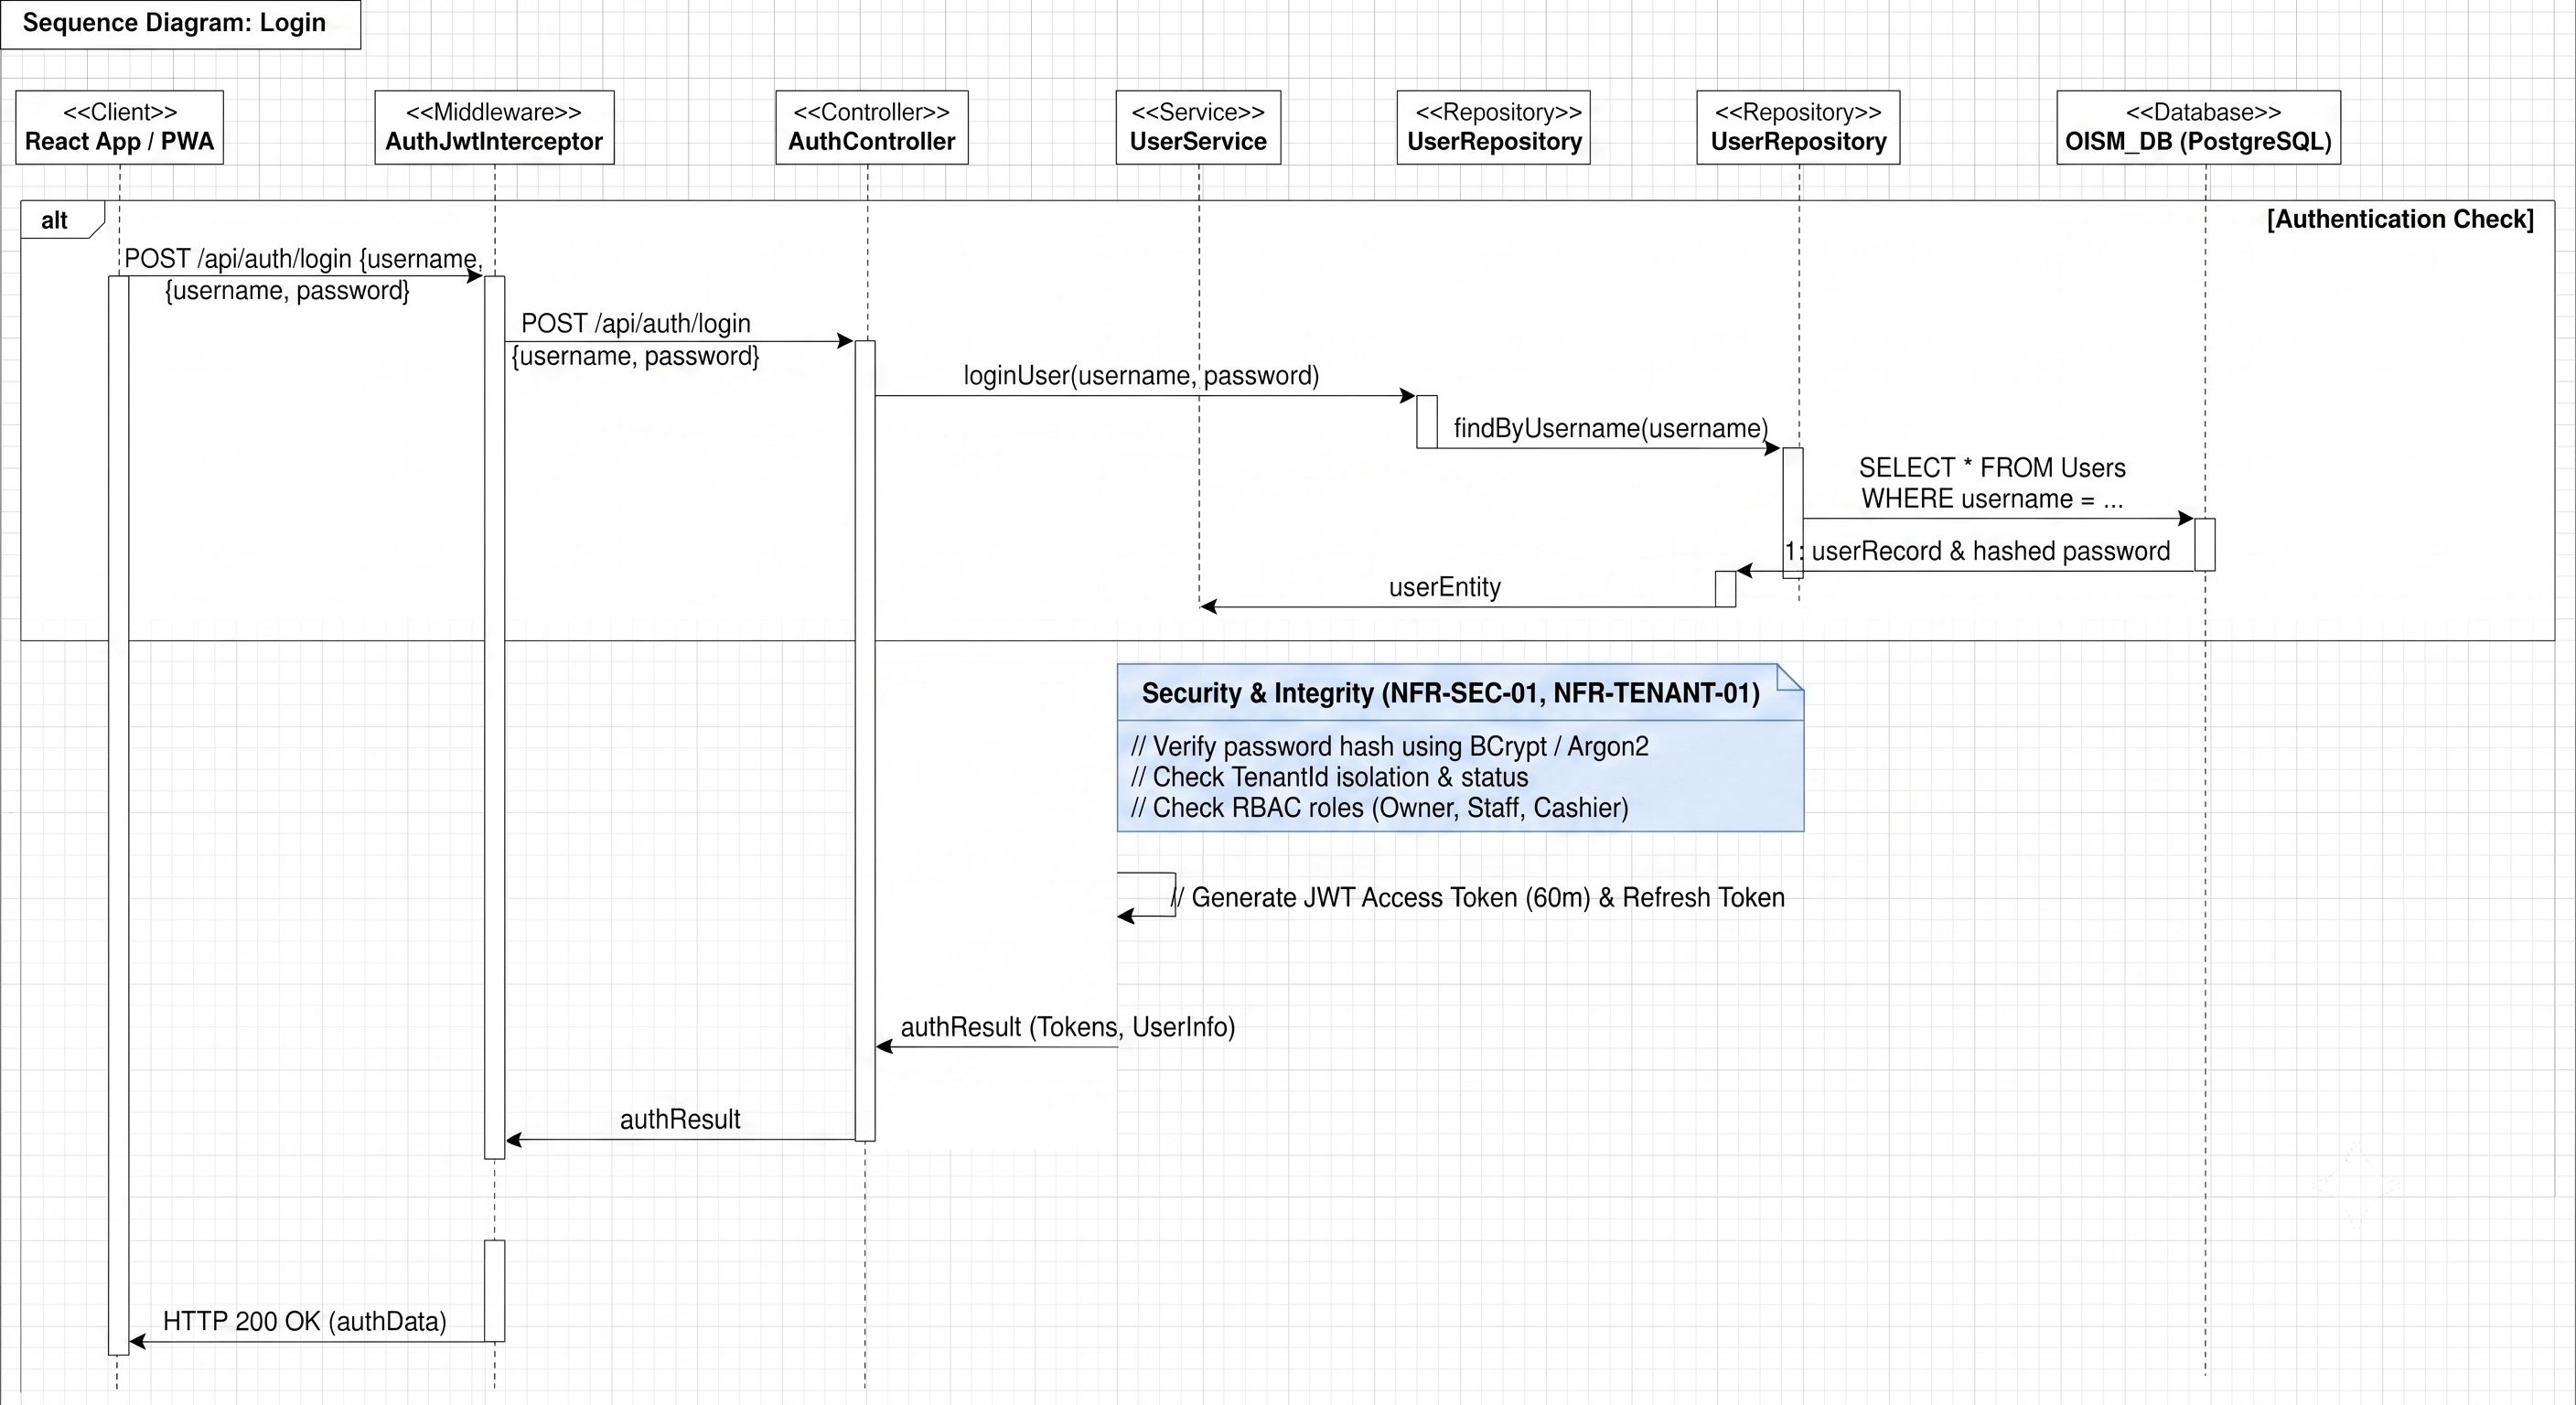
\includegraphics[width=0.88\textwidth]{Login.png}
		\caption{Sequence Diagram: Luồng Đăng nhập hệ thống}
	\end{figure}
	\begin{figure}[H]
		\centering
		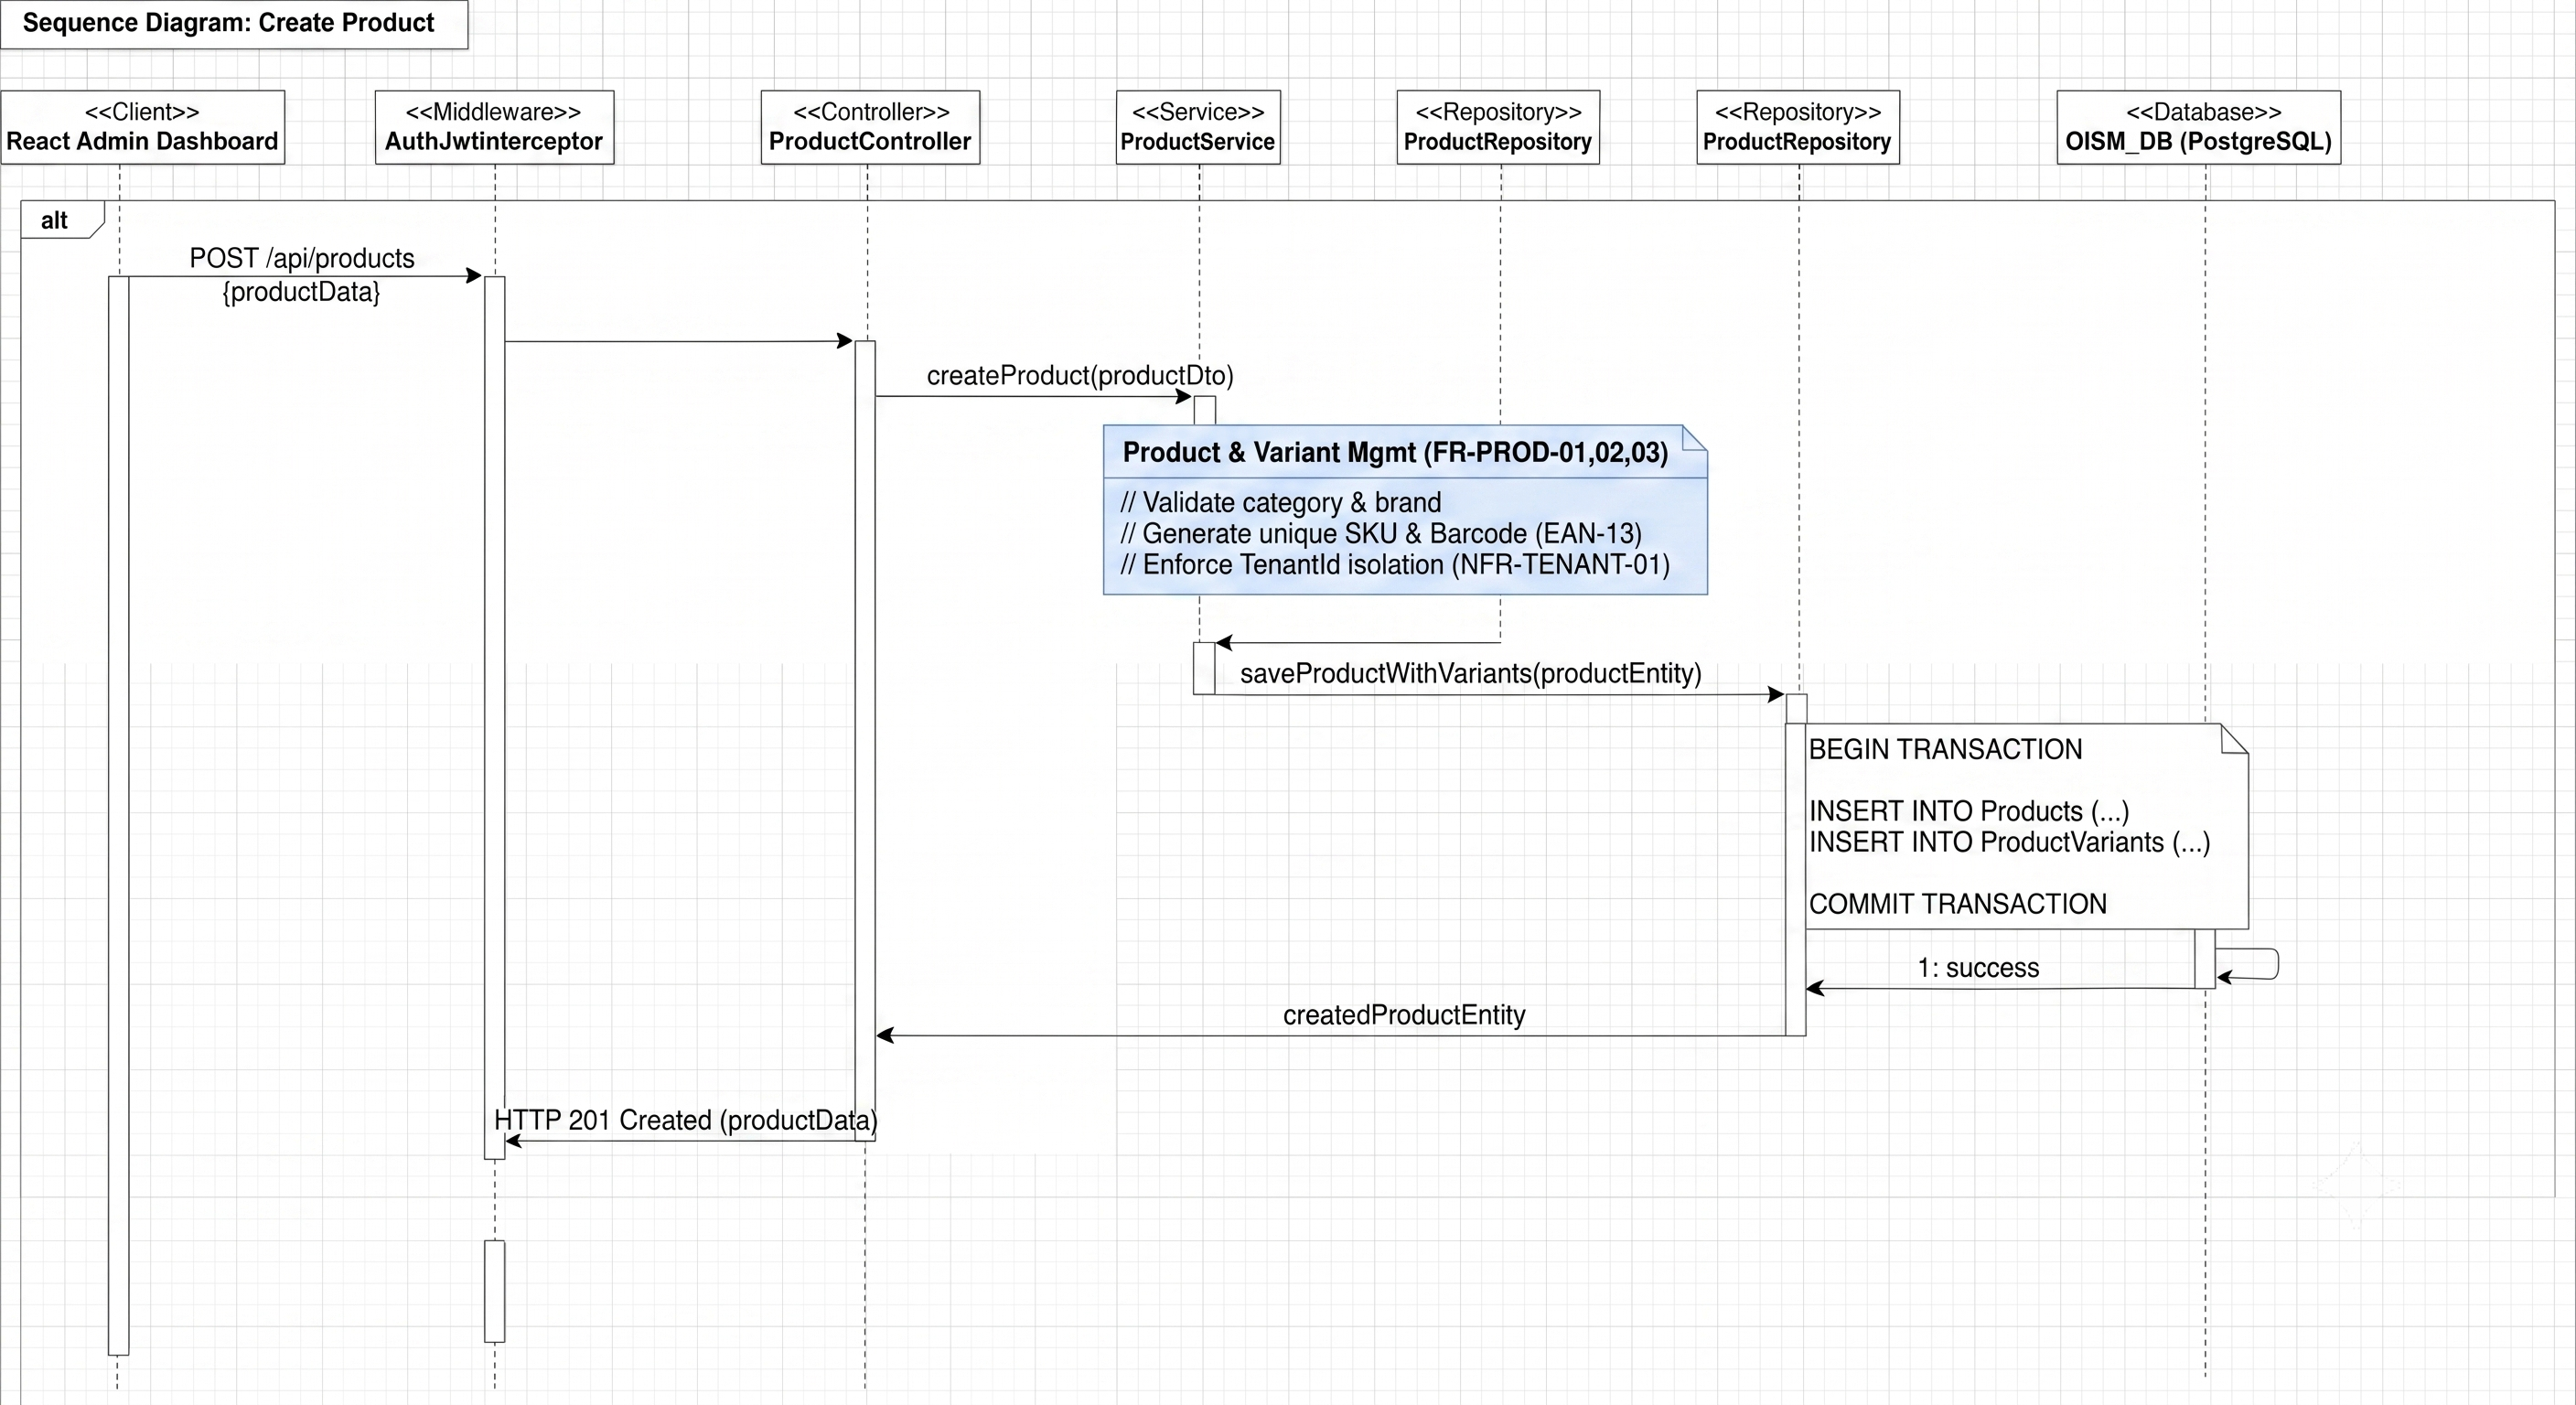
\includegraphics[width=0.88\textwidth]{Create Product.png}
		\caption{Sequence Diagram: Luồng Tạo sản phẩm}
	\end{figure}
	\begin{figure}[H]
		\centering
		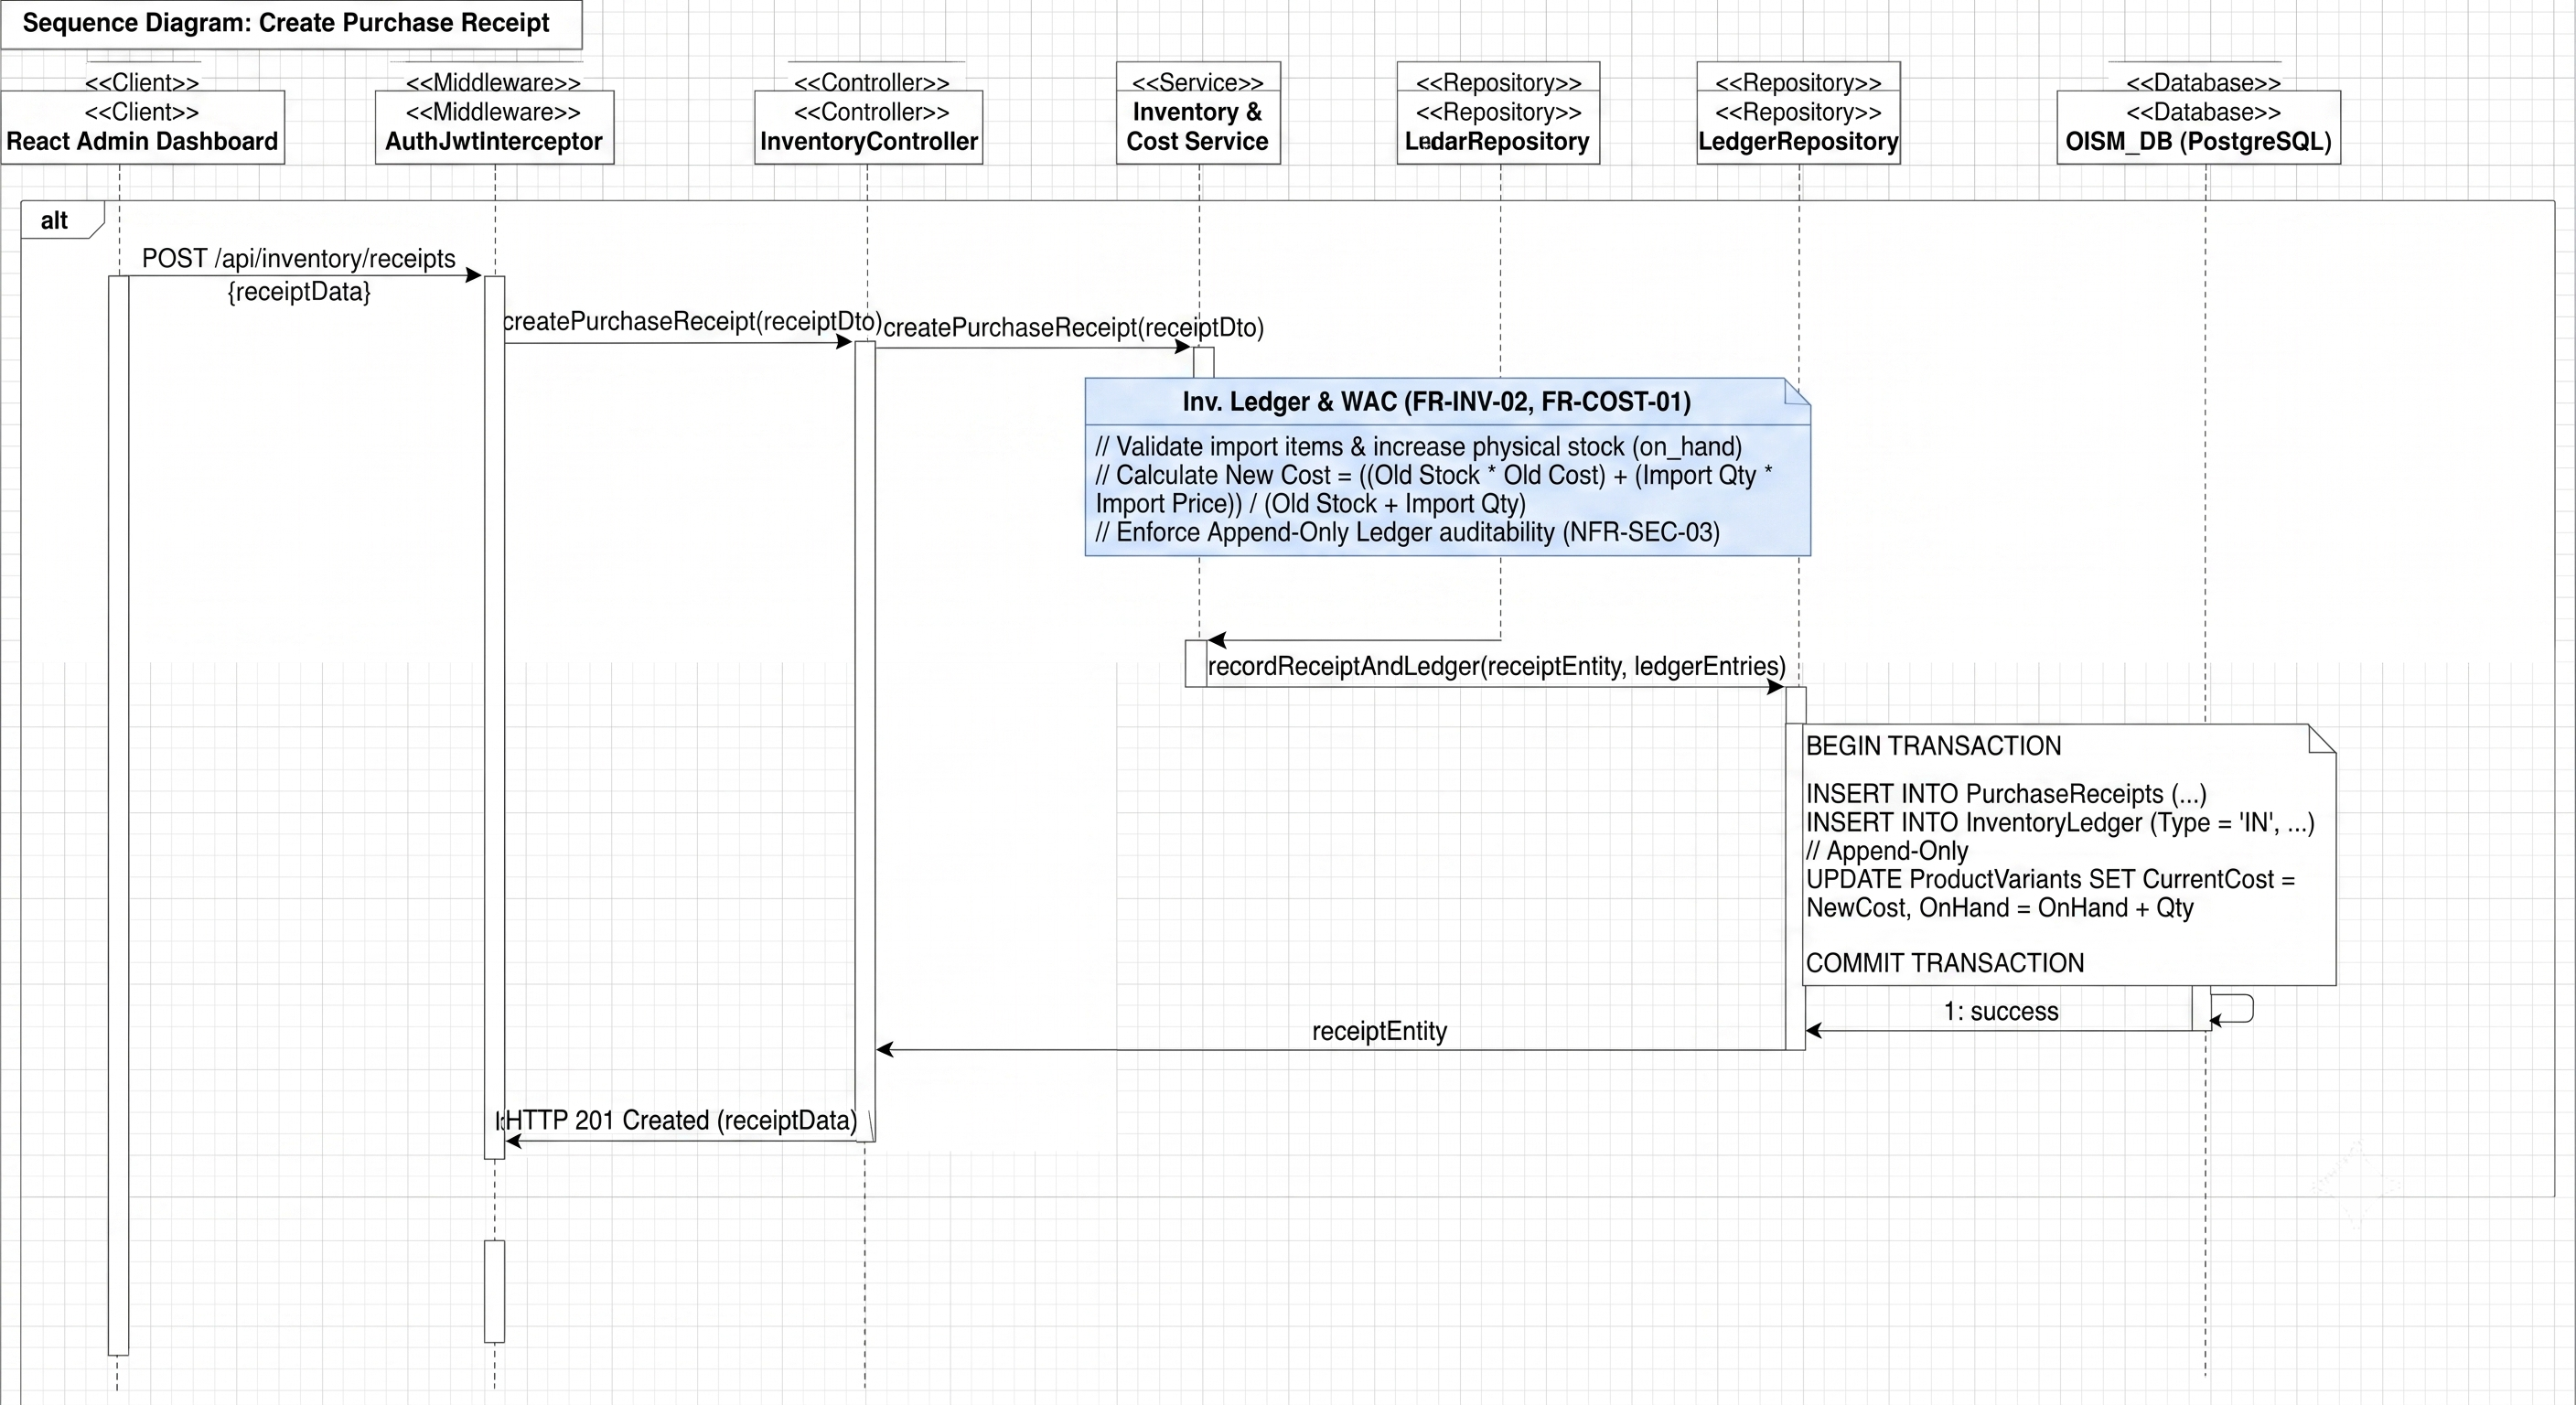
\includegraphics[width=0.88\textwidth]{Create Receipt.png}
		\caption{Sequence Diagram: Luồng Lập phiếu nhập kho}
	\end{figure}
	\begin{figure}[H]
		\centering
		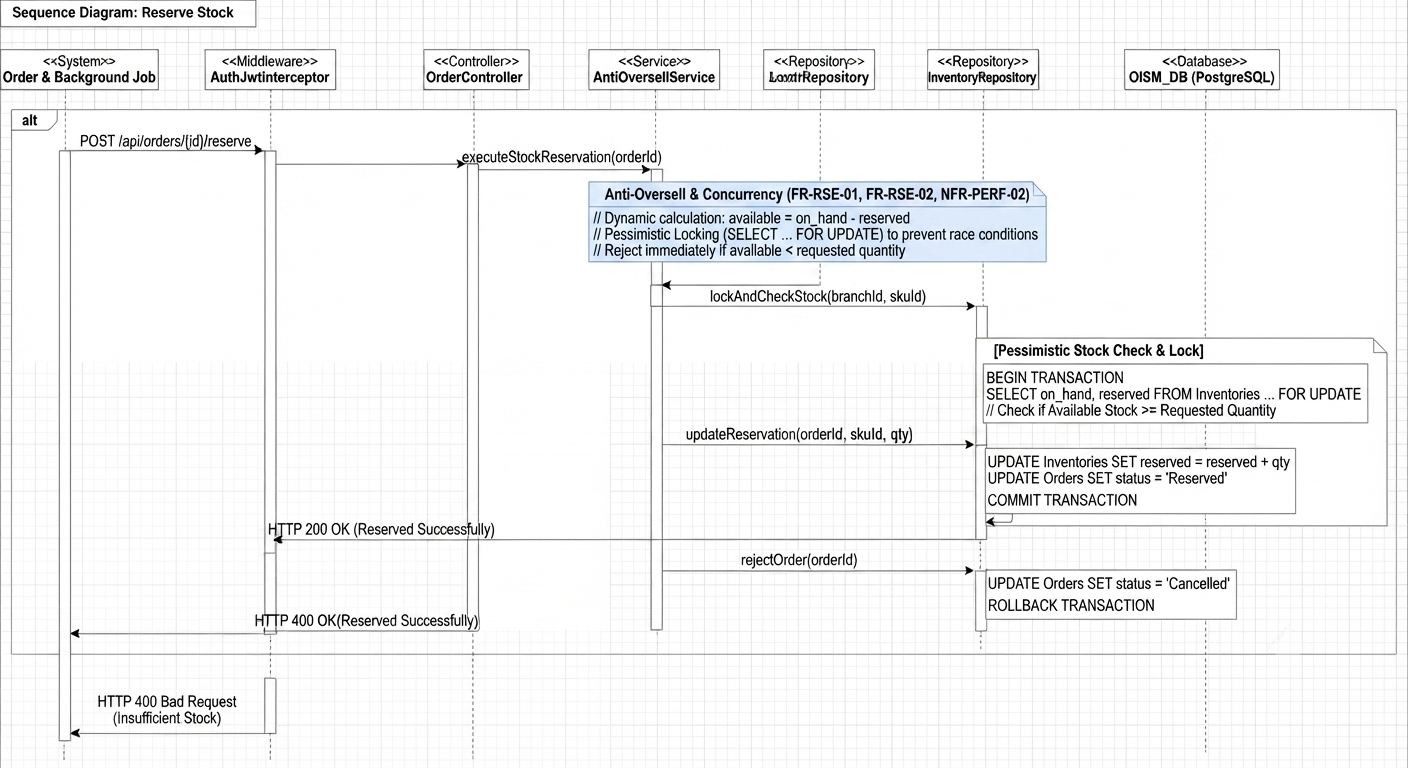
\includegraphics[width=0.88\textwidth]{Reserve Stock.png}
		\caption{Sequence Diagram: Luồng Giữ chỗ tồn kho}
	\end{figure}
	\begin{figure}[H]
		\centering
		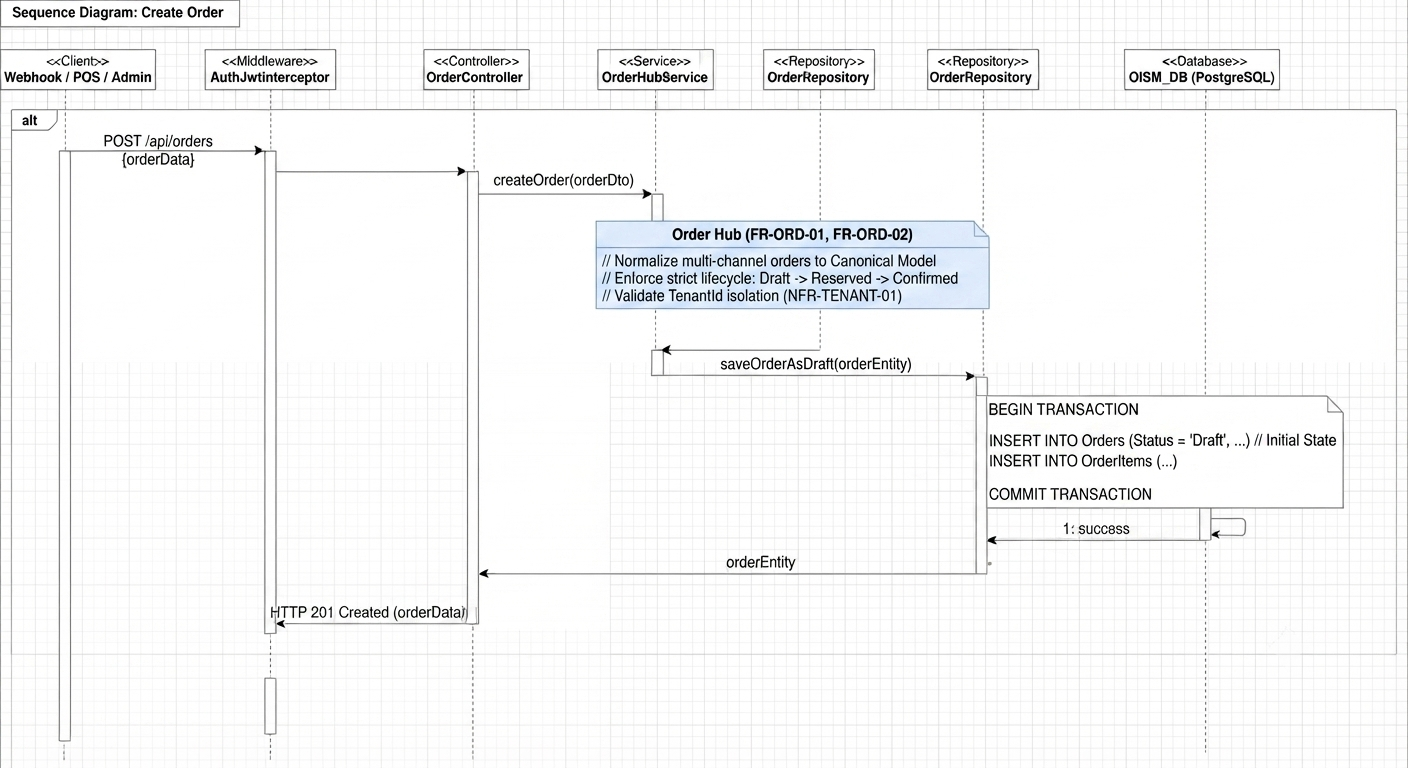
\includegraphics[width=0.88\textwidth]{Create Order.png}
		\caption{Sequence Diagram: Luồng Tạo đơn hàng}
	\end{figure}
	\begin{figure}[H]
		\centering
		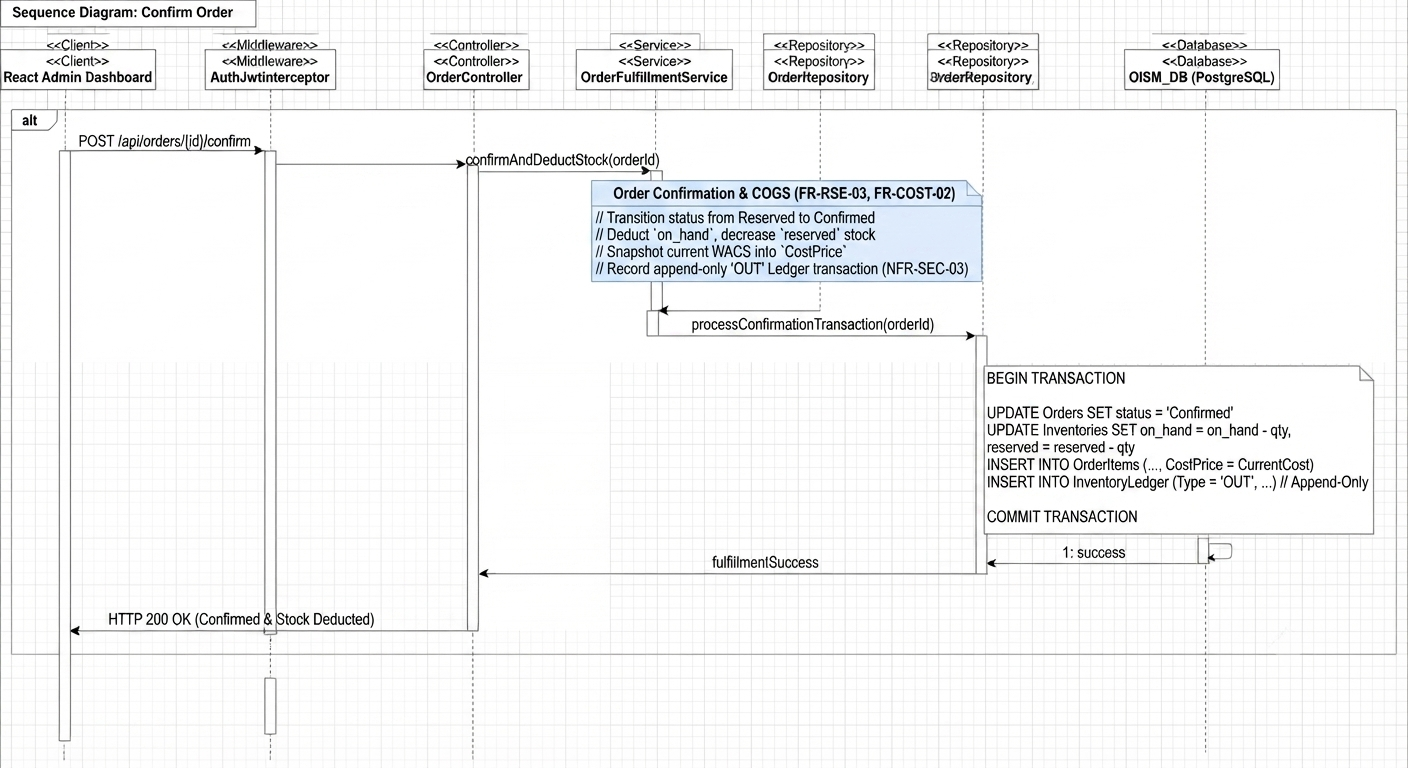
\includegraphics[width=0.88\textwidth]{Confirm Order.png}
		\caption{Sequence Diagram: Luồng Xác nhận đơn hàng}
	\end{figure}
	\begin{figure}[H]
		\centering
		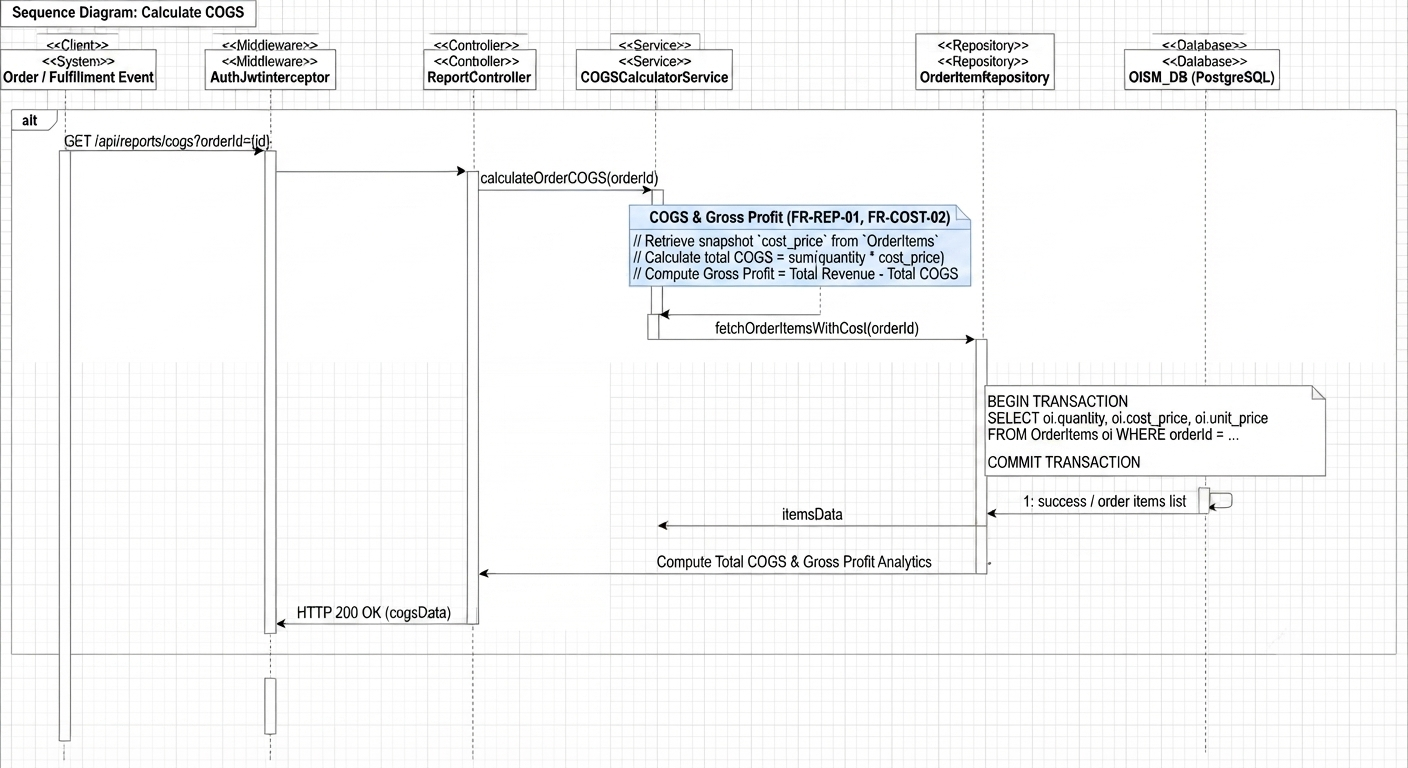
\includegraphics[width=0.88\textwidth]{Calculate COGS.png}
		\caption{Sequence Diagram: Luồng Tính toán Giá vốn}
	\end{figure}
	\begin{figure}[H]
		\centering
		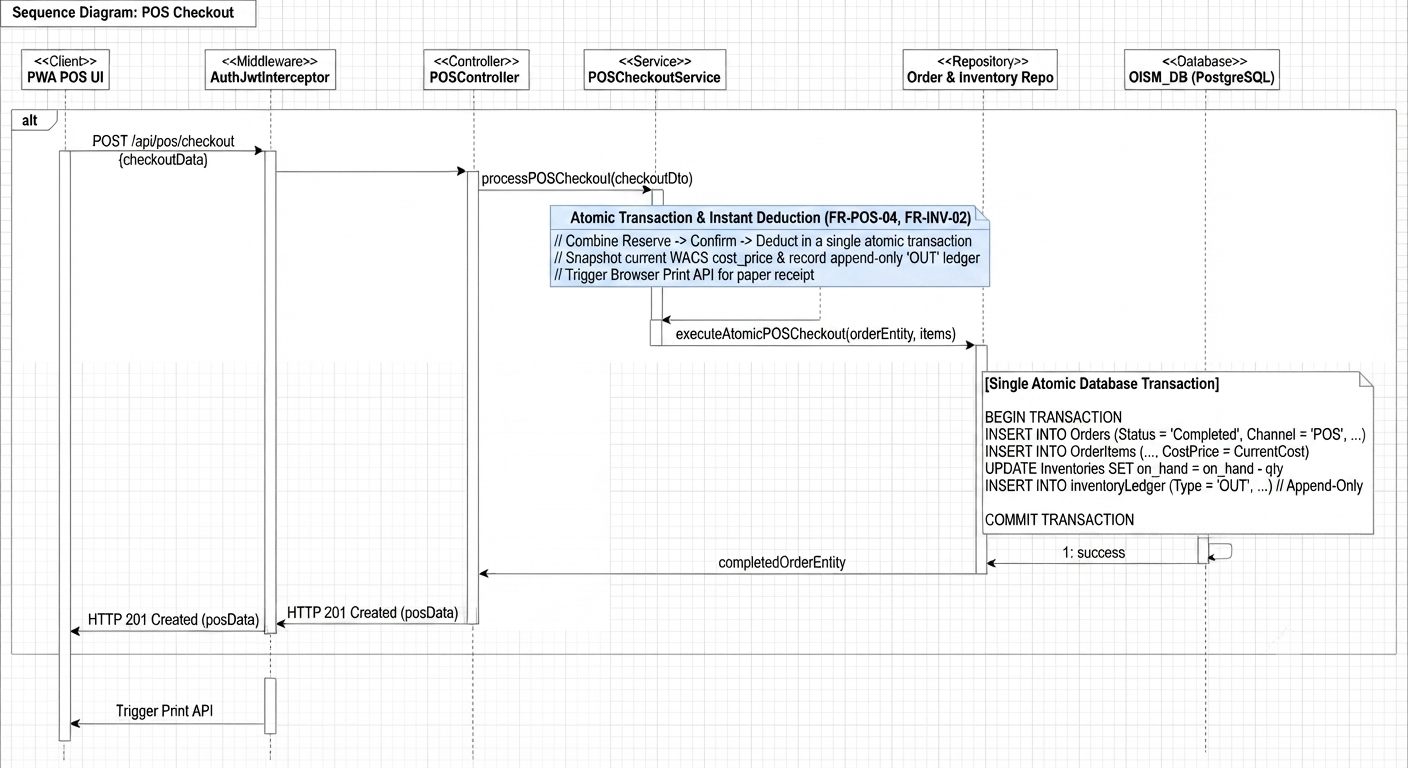
\includegraphics[width=0.88\textwidth]{POS Checkout.png}
		\caption{Sequence Diagram: Luồng Thanh toán POS}
	\end{figure}
	
	\section{Thiết kế Anti-Oversell}
	Bài toán chống bán quá tải (Anti-Oversell) là một trong những thách thức kỹ thuật cốt lõi và phức tạp nhất đối với các hệ thống thương mại điện tử đa kênh và bán lẻ phân tán. Khi diễn ra các sự kiện khuyến mãi lớn hoặc chiến dịch Flash Sale, hàng nghìn khách hàng có thể cùng lúc thực hiện thao tác đặt mua một mặt hàng SKU có số lượng giới hạn. Nếu hệ thống không trang bị cơ chế kiểm soát đồng thời hiệu quả, hiện tượng tranh chấp dữ liệu sẽ xảy ra, dẫn đến việc nhiều đơn hàng được chấp nhận vượt quá tổng lượng tồn kho thực tế, gây thất thoát tài chính và làm suy giảm uy tín nghiêm trọng của doanh nghiệp.
	\par
	Để giải quyết triệt để bài toán này, hệ thống OISM xây dựng mô hình kiểm soát tồn kho khả dụng dựa trên công thức cốt lõi: 
	\begin{equation*}
		\text{Available} = \text{OnHand} - \text{Reserved}
	\end{equation*}
	Trong đó, \textit{OnHand} biểu thị số lượng hàng tồn kho vật lý thực tế đang nằm trong kho của chi nhánh, và \textit{Reserved} là số lượng hàng hóa đã được giữ chỗ tạm thời (Reservation) trong các đơn hàng trực tuyến đang chờ xác nhận hoặc chờ thanh toán. 
	\par
	Về mặt hiện thực kỹ thuật, khi một đơn hàng trực tuyến được đẩy vào hệ thống, cỗ máy xử lý đơn hàng sẽ kích hoạt giao dịch cơ sở dữ liệu ở mức cô lập cao (\textit{Repeatable Read / Serializable}), kết hợp sử dụng câu lệnh khóa dòng (\textit{SELECT SKU WHERE Id = ? FOR UPDATE}) trên bảng lưu trữ biến thể sản phẩm. Cơ chế này buộc các luồng giao dịch đồng thời từ nhiều kênh khác nhau phải xếp hàng tuần tự theo hàng đợi của cơ sở dữ liệu, đảm bảo rằng việc kiểm tra điều kiện tồn kho khả dụng và tăng số lượng giữ chỗ (\textit{Reserved}) diễn ra bên trong một khối giao dịch nguyên tử (Atomic Transaction) khép kín tuyệt đối, từ đó loại bỏ hoàn toàn khả năng phát sinh tồn kho âm.
	
	\section{Thiết kế POS}
	Phân hệ bán hàng tại quầy (POS) đóng vai trò là cầu nối vận hành chiến lược, phục vụ trực tiếp cho đội ngũ thu ngân tại các cửa hàng vật lý. Hệ thống được phát triển theo mô hình ứng dụng web tiến bộ (Progressive Web App - PWA), mang lại trải nghiệm mượt mà, tốc độ phản hồi tối ưu và khả năng tương thích cao trên nhiều định dạng phần cứng khác nhau, từ máy tính để bàn truyền thống, máy tính bảng đến các thiết bị POS cầm tay chuyên dụng.
	\par
	Giao diện POS được thiết kế theo hướng tối giản hóa thao tác cảm ứng, hỗ trợ tính năng tra cứu sản phẩm siêu tốc thông qua tên gọi, mã định danh SKU hoặc quét mã vạch trực tiếp qua thiết bị đọc barcode USB/Camera. Ngay tại thời điểm thu ngân thêm sản phẩm vào giỏ hàng, hệ thống thực hiện truy vấn tức thời để xác thực tồn kho khả dụng tại chi nhánh hiện tại, chặn đứng các giao dịch vượt mức tồn kho để bảo vệ lượng phân bổ giữ chỗ dành cho kênh trực tuyến. Quy trình thanh toán được chuẩn hóa thành một thao tác nguyên tử duy nhất: vừa tạo đơn hàng, vừa trừ kho vật lý, vừa ghi nhận bút toán sổ cái bất biến và tự động kích hoạt hộp thoại gọi lệnh in hóa đơn thông qua trình duyệt (\textit{Browser Print API}).
	
	\section{Thiết kế Real-time và Background Processing}
	Trong môi trường bán lẻ đa kênh thời gian thực, việc cập nhật thông tin trạng thái đơn hàng tức thời và tự động hóa các tác vụ nền đóng vai trò quyết định đến hiệu suất vận hành và trải nghiệm của người quản lý.
	\par
	\begin{itemize}
		\item \textbf{Xử lý thời gian thực với SignalR:} Hệ thống tích hợp công nghệ WebSockets thông qua thư viện SignalR phía Backend, thiết lập kênh kết nối hai chiều liên tục giữa máy chủ và giao diện người dùng. Khi có một đơn hàng mới từ sàn thương mại điện tử đổ về qua Webhook hoặc có thay đổi trạng thái giao dịch từ quầy POS, máy chủ sẽ tự động đẩy thông báo âm thanh và popup trực tiếp đến màn hình của quản trị viên và nhân viên kho mà không yêu cầu người dùng phải thực hiện thao tác tải lại trang (F5).
		\item \textbf{Tác vụ nền với Hangfire:} Đối với các công việc nặng tính toán hoặc mang tính chu kỳ (như tự động hủy các đơn hàng giữ chỗ quá hạn thanh toán sau một khoảng thời gian quy định, tổng hợp số liệu doanh thu cuối ngày, đồng bộ dữ liệu tồn kho định kỳ), hệ thống sử dụng thư viện Hangfire để lập lịch và thực thi ngầm an toàn, đảm bảo không làm ảnh hưởng đến tốc độ phản hồi của các API phục vụ trực tiếp cho khách hàng.
	\end{itemize}
	
	\section{Thiết kế AI}
	Nhằm nâng cao năng lực cạnh tranh và hỗ trợ đắc lực cho nhà quản trị trong công tác ra quyết định chiến lược, hệ thống OISM tích hợp phân hệ phân tích thông minh dựa trên việc khai thác dữ liệu lịch sử giao dịch.
	\par
	Module AI đảm nhiệm việc phân tích tốc độ luân chuyển của từng mặt hàng SKU (\textit{Inventory Velocity}), từ đó tự động phân nhóm hàng hóa theo mô hình ABC/XYZ, nhận diện các mặt hàng bán chạy (Best-sellers) và các mặt hàng tồn kho chậm luân chuyển (Dead stock). Dựa trên các chỉ số này, hệ thống cung cấp các biểu đồ trực quan và đưa ra các gợi ý đề xuất tự động về thời điểm cũng như số lượng cần nhập hàng bổ sung cho từng nhà cung cấp, giúp doanh nghiệp tối ưu hóa nguồn vốn lưu động và hạn chế tình trạng ứ đọng hàng tồn kho.
	
	% ============================================================
	% CHƯƠNG 5. KIỂM THỬ PHẦN MỀM
	% ============================================================
	\chapter{KIỂM THỬ PHẦN MỀM}
	\section{Phạm vi kiểm thử}
	Thực hiện kiểm thử toàn diện các chức năng nghiệp vụ, tính bảo mật phân quyền, khả năng cô lập dữ liệu tenant và hiệu năng chịu tải của toàn bộ hệ thống.
	
	\section{Chiến lược kiểm thử}
	Kết hợp đồng bộ giữa kiểm thử đơn vị (Unit Test), kiểm thử tích hợp (Integration Test), kiểm thử hệ thống (System Test) và kiểm thử đồng thời (Concurrency Test).
	
	\section{Môi trường kiểm thử}
	Triển khai thực thi kiểm thử trên môi trường giả lập cục bộ và môi trường staging trên đám mây để đảm bảo độ tin cậy tương đương production.
	
	\section{Kế hoạch kiểm thử}
	Lịch trình phân bổ các mốc milestone kiểm thử bám sát giai đoạn nước rút từ tuần thứ 11 đến tuần thứ 15 của đồ án.
	
	\section{Unit Test}
	Tập trung kiểm định tính chính xác của các hàm tính toán giá vốn WAC và công thức xác định tồn kho khả dụng.
	
	\section{Integration Test}
	Kiểm tra sự tương thích và truyền tải dữ liệu chính xác giữa các tầng API Controller, Business Service và cơ sở dữ liệu PostgreSQL.
	
	\section{System Test}
	Kiểm thử toàn vẹn các luồng nghiệp vụ khép kín End-to-End từ khâu tiếp nhận đơn hàng, giữ chỗ đến khi thanh toán thành công.
	
	\section{Performance Test}
	Đánh giá mức độ đáp ứng thời gian phản hồi của hệ thống dưới các ngưỡng tải giao dịch khác nhau.
	
	\section{Concurrency Test}
	Thực hiện kịch bản kiểm thử đồng thời giả lập 50 luồng request cùng tranh chấp 1 mặt hàng SKU duy nhất trong điều kiện số lượng có hạn.
	
	\section{Security Test}
	Xác thực mức độ an toàn của mã thông báo JWT, tính hiệu quả của phân quyền RBAC và cơ chế ngăn chặn rò rỉ dữ liệu giữa các tenant.
	
	\section{Test Case}
	Tổng hợp chi tiết danh sách các kịch bản kiểm thử cho từng module chức năng cụ thể trong hệ thống.
	
	\section{Kết quả kiểm thử}
	Ghi nhận kết quả thực tế vượt qua các tập lệnh kiểm thử tự động (\texttt{smoke\_test.py}, \texttt{e2e\_local.py}).
	
	\section{Phân tích lỗi}
	Đánh giá các vấn đề phát sinh trong quá trình kiểm thử và đưa ra phương án khắc phục triệt để.
	
	% ============================================================
	% CHƯƠNG 6. ĐÓNG GÓI, TRIỂN KHAI VÀ HƯỚNG DẪN SỬ DỤNG
	% ============================================================
	\chapter{ĐÓNG GÓI, TRIỂN KHAI VÀ HƯỚNG DẪN SỬ DỤNG}
	\section{Các sản phẩm bàn giao}
	Hệ thống bàn giao bao gồm mã nguồn Backend .NET 8, ứng dụng Admin Dashboard, giao diện POS PWA, cơ sở dữ liệu PostgreSQL kèm dữ liệu mẫu, trọn bộ tài liệu kỹ thuật và gói Docker Compose.
	
	\section{Yêu cầu hệ thống}
	Bảng tổng hợp cấu hình phần cứng và phần mềm tối thiểu để triển khai vận hành hệ thống:
	\begin{table}[H]
		\centering
		\caption{Bảng yêu cầu cấu hình hệ thống triển khai}
		\begin{tabularx}{\textwidth}{p{0.25\textwidth} p{0.35\textwidth} p{0.35\textwidth}}
			\toprule
			\textbf{Thành phần} & \textbf{Tối thiểu} & \textbf{Khuyến nghị}\\
			\midrule
			CPU & Multi-core 1.8 GHz & Multi-core 2.4 GHz trở lên\\
			RAM & 4 GB & 8 GB trở lên\\
			Storage & 128 GB SSD & 256 GB SSD trở lên\\
			OS & Windows 10 / Ubuntu 20.04 & Windows 11 / Ubuntu 22.04\\
			Browser & Chrome / Edge phiên bản cũ & Chrome / Edge bản mới nhất\\
			Docker & Phiên bản hỗ trợ Compose & Phiên bản ổn định mới nhất\\
			.NET / Python & .NET 8 / Python 3.10 & .NET 8 / Python 3.11\\
			\bottomrule
		\end{tabularx}
	\end{table}
	
	\section{Hướng dẫn cài đặt}
	Chi tiết các bước chuẩn bị môi trường, tải mã nguồn, cấu hình biến môi trường và khởi chạy các dịch vụ thành phần trên máy cục bộ.
	
	\section{Hướng dẫn triển khai Docker}
	Mô tả cấu trúc đóng gói container thông qua Docker Compose giúp tự động hóa hoàn toàn quá trình dựng cờ môi trường triển khai.
	
	\section{Hướng dẫn sử dụng Owner}
	Tài liệu hướng dẫn thao tác chi tiết dành cho chủ cửa hàng từ việc đăng nhập, quản lý nhân sự, danh mục sản phẩm đến theo dõi báo cáo lợi nhuận gộp.
	
	\section{Hướng dẫn sử dụng Staff}
	Hướng dẫn nghiệp vụ cho nhân viên kho thực hiện lập phiếu nhập hàng, điều chuyển kho và xử lý đơn hàng đa kênh.
	
	\section{Hướng dẫn sử dụng Cashier}
	Quy trình thao tác bán hàng nhanh tại quầy dành cho thu ngân sử dụng giao diện PWA POS.
	
	\section{API Documentation}
	Tài liệu đặc tả toàn bộ các RESTful API tích hợp sẵn giao diện Swagger UI phục vụ công tác tích hợp và kiểm thử.
	
	\section{Repository và CI/CD}
	Thông tin về kho lưu trữ mã nguồn trên GitHub và cơ chế tự động hóa quy trình CI/CD qua GitHub Actions.
	
	% ============================================================
	% KẾT LUẬN
	% ============================================================
	\chapter*{KẾT LUẬN}
	\addcontentsline{toc}{chapter}{KẾT LUẬN}
	Đồ án đã hoàn thành việc nghiên cứu, thiết kế và hiện thực hóa thành công hệ thống Quản lý Bán hàng và Tồn kho Đa kênh (OISM). Hệ thống giải quyết triệt để các bài toán cốt lõi của bán lẻ hiện đại như chống bán quá tải (Anti-Oversell), tính toán giá vốn tự động theo phương pháp bình quân gia quyền và đảm bảo tính minh bạch thông qua sổ cái tồn kho bất biến. 
	
	Với việc ứng dụng Clean Architecture và mô hình SaaS đa thuê bao, OISM sở hữu khả năng mở rộng mạnh mẽ, tính bảo mật cao và sẵn sàng đáp ứng các tiêu chuẩn vận hành thực tế của doanh nghiệp.
	
	% ============================================================
	% TÀI LIỆU THAM KHẢO
	% ============================================================
	\chapter*{TÀI LIỆU THAM KHẢO}
	\addcontentsline{toc}{chapter}{TÀI LIỆU THAM KHẢO}
	\begin{enumerate}
		\item Tài liệu hướng dẫn đồ án Capstone Project do Khoa CNTT - ĐH GTVT TP.HCM cung cấp.
		\item Tài liệu đề xuất dự án Omnichannel Inventory and Sales Management System (OISM).
		\item Source code và test suite của nhóm dự án OISM2.
	\end{enumerate}

\end{document}